\documentclass[12pt,a4paper]{article}

% -------------------------------------------------------------------
%  Packages
% -------------------------------------------------------------------
\usepackage[T1]{fontenc}
\usepackage[utf8]{inputenc}
\usepackage{lmodern}
\usepackage{microtype}
\usepackage{geometry}
\geometry{margin=2.5cm}
\usepackage{amsmath,amssymb}
\usepackage{booktabs}
\usepackage{graphicx}
\usepackage{float}
\usepackage{hyperref}
\usepackage{cleveref}
\usepackage{caption}
\usepackage{subcaption}
\usepackage{xcolor}
\usepackage{array}
\usepackage{longtable}

% -------------------------------------------------------------------
%  Metadata
% -------------------------------------------------------------------
\title{%
  \textbf{IC-Knockoff-PolyReg: Simulation Study}\\[6pt]
  \large Polynomial Regression with Knockoff-Based FDR Control
}
\author{Simulation Report --- Auto-generated}
\date{\today}

% ===================================================================
\begin{document}
\maketitle
\tableofcontents
\newpage

% ===================================================================
\section{Introduction}
\label{sec:intro}

This report summarises the Monte-Carlo simulation study for
\textbf{IC-Knockoff-PolyReg} (IC-Knock-Poly), a method that combines
iterative conformalisation of knockoff statistics with polynomial
dictionary regression to perform simultaneous feature selection and
prediction under FDR control.

The method is evaluated on synthetically generated datasets where the
ground-truth response is a \(k\)-sparse polynomial of \(p\) base features
drawn from a Gaussian Mixture Model (GMM).
Two complementary sweeps are performed:

\begin{itemize}
  \item \textbf{Default sweep}: fixes \(p=5\) base features and varies
        sample size \(n \in \{100, 300, 500\}\), sparsity \(k \in \{2,3\}\),
        and evaluation setting (\emph{supervised} vs.\ \emph{semi-supervised})
        at polynomial degree \(d=2\).
        All six competing methods are compared.
  \item \textbf{Degree\,$\times$\,non-zero sweep}: fixes \(p=5\) and sweeps
        polynomial degree \(d \in \{2,3\}\) together with the number of
        non-zero elements \(k \in \{2,3,4\}\) at two sample sizes.
\end{itemize}

\noindent\textbf{Computational note.}
IC-Knock-Poly's runtime grows steeply with \(p\) because the
Model-X knockoff construction requires solving a semidefinite programme
over the \(p \cdot d \times p \cdot d\) polynomial-term covariance matrix.
All experiments therefore fix \(p = 5\); larger \(p\) experiments
can be run on more powerful hardware by adjusting the parameters in
\texttt{run\_simulations.py}.

Figures are generated by \texttt{simulations/visualize.py} and saved as
PDF vector graphics.  Numerical results are archived in
\texttt{default\_sweep\_summary.json} and
\texttt{degree\_nonzero\_sweep\_summary.json}.

% ===================================================================
\section{Experimental Setup}
\label{sec:setup}

\subsection{Data-Generating Process}

Each dataset is drawn from:
\begin{align}
  X       &\sim \mathrm{GMM}\!\left(K=2,\; p=5\right), \notag\\
  y       &= \Phi(X)^\top \beta^* + \varepsilon, \quad
             \varepsilon \sim \mathcal{N}(0, \sigma^2 = 0.25),\notag
\end{align}
where \(\Phi(\cdot)\) is the rational polynomial dictionary of degree \(d\)
(terms \(x_j^1, x_j^2, \ldots, x_j^d, x_j^{-1}, \ldots, x_j^{-d}\) for
each base feature \(x_j\)), and \(\beta^*\) is \(k\)-sparse with non-zero
coefficients drawn uniformly from \([-2,-0.5]\cup[0.5,2]\).

\subsection{Competing Methods}

\begin{description}
  \item[\textbf{IC-Knock-Poly}] (proposed method)
    Iterative conformal knockoff procedure with GMM-estimated covariate
    model and polynomial dictionary; controlled at FDR level \(Q=0.10\).
  \item[\textbf{Poly-Lasso}]
    LASSO regression on the full polynomial dictionary; threshold chosen
    by cross-validation.
  \item[\textbf{Poly-OMP}]
    Orthogonal Matching Pursuit on the polynomial dictionary; sparsity
    set to the estimated non-zero count.
  \item[\textbf{Poly-CLIME}]
    Constrained \(\ell_1\)-minimisation for inverse covariance estimation
    combined with polynomial regression.
  \item[\textbf{Poly-Knockoff}]
    Model-X knockoffs applied directly to the polynomial dictionary.
  \item[\textbf{Sparse-Poly-STLSQ}]
    Sequentially thresholded least-squares on the polynomial dictionary.
\end{description}

\subsection{Evaluation Metrics}

\begin{itemize}
  \item \textbf{FDR}: empirical false discovery rate
        \(= \mathrm{FP}/\max(1,\mathrm{FP}+\mathrm{TP})\).
  \item \textbf{TPR / Recall}: true positive rate
        \(= \mathrm{TP}/(\mathrm{TP}+\mathrm{FN})\).
  \item \textbf{Precision}: \(= \mathrm{TP}/\max(1,\mathrm{TP}+\mathrm{FP})\).
  \item \textbf{F1}: harmonic mean of precision and recall.
  \item \textbf{AUC}: approximate area under the ROC curve
        \(= 0.5(\mathrm{TPR} + \mathrm{TNR})\).
  \item \textbf{R\textsuperscript{2}}: coefficient of determination on
        the labeled data.
\end{itemize}

All metrics are averaged over 3 independent trials.
Target FDR level: \(Q = 0.10\);
noise: \(\sigma = 0.5\);
maximum iterations for IC-Knock-Poly: 10.

% ===================================================================
\section{Default Sweep Results}
\label{sec:default}

\subsection{Summary Table}

\Cref{tab:default} reports the aggregate performance metrics for every
configuration in the default sweep.


\begin{table}[htbp]
\centering
\caption{Default sweep results ($p=5$, degree $d=2$). Mean FDR, TPR, F1, AUC, R\textsuperscript{2}, and wall-clock time over completed trials.}
\label{tab:default}
\resizebox{\textwidth}{!}{%
\begin{tabular}{llccccccc}
\hline
\textbf{Config} & \textbf{Method} & \textbf{FDR} & \textbf{TPR} &
\textbf{F1} & \textbf{AUC} & \textbf{R\textsuperscript{2}} & \textbf{Time (s)} & \textbf{Trials} \\
\hline
  p5\_n100\_k2\_d2\_supervised & ic\_knock\_poly & 0.000 & 0.000 & 0.000 & 0.500 & 0.000 & 12.09 & 3 \\
  p5\_n100\_k2\_d2\_supervised & poly\_lasso & 0.444 & 1.000 & 0.711 & 0.722 & 0.979 & 0.22 & 3 \\
  p5\_n100\_k2\_d2\_supervised & poly\_omp & 0.222 & 1.000 & 0.867 & 0.889 & 0.980 & 0.02 & 3 \\
  p5\_n100\_k2\_d2\_supervised & poly\_clime & 0.000 & 0.000 & 0.000 & 0.500 & 0.979 & 0.39 & 3 \\
  p5\_n100\_k2\_d2\_supervised & poly\_knockoff & 0.000 & 0.000 & 0.000 & 0.500 & 0.979 & 0.23 & 3 \\
  p5\_n100\_k2\_d2\_supervised & sparse\_poly\_stlsq & 0.111 & 1.000 & 0.933 & 0.944 & 0.982 & 0.01 & 3 \\
  p5\_n100\_k2\_d2\_semi\_supervised & ic\_knock\_poly & 0.000 & 0.000 & 0.000 & 0.500 & 0.000 & 5.12 & 3 \\
  p5\_n100\_k2\_d2\_semi\_supervised & poly\_lasso & 0.367 & 1.000 & 0.746 & 0.722 & 0.978 & 0.21 & 3 \\
  p5\_n100\_k2\_d2\_semi\_supervised & poly\_omp & 0.200 & 1.000 & 0.857 & 0.833 & 0.978 & 0.02 & 3 \\
  p5\_n100\_k2\_d2\_semi\_supervised & poly\_clime & 0.000 & 0.000 & 0.000 & 0.500 & 0.975 & 0.31 & 3 \\
  p5\_n100\_k2\_d2\_semi\_supervised & poly\_knockoff & 0.000 & 0.000 & 0.000 & 0.500 & 0.974 & 0.23 & 3 \\
  p5\_n100\_k2\_d2\_semi\_supervised & sparse\_poly\_stlsq & 0.478 & 1.000 & 0.679 & 0.667 & 0.979 & 0.01 & 3 \\
  p5\_n100\_k3\_d2\_supervised & ic\_knock\_poly & 0.000 & 0.000 & 0.000 & 0.500 & 0.000 & 11.83 & 3 \\
  p5\_n100\_k3\_d2\_supervised & poly\_lasso & 0.083 & 1.000 & 0.952 & 0.917 & 0.979 & 0.22 & 3 \\
  p5\_n100\_k3\_d2\_supervised & poly\_omp & 0.217 & 1.000 & 0.869 & 0.750 & 0.983 & 0.03 & 3 \\
  p5\_n100\_k3\_d2\_supervised & poly\_clime & 0.000 & 0.000 & 0.000 & 0.500 & 0.869 & 0.40 & 3 \\
  p5\_n100\_k3\_d2\_supervised & poly\_knockoff & 0.000 & 0.000 & 0.000 & 0.500 & 0.977 & 0.24 & 3 \\
  p5\_n100\_k3\_d2\_supervised & sparse\_poly\_stlsq & 0.167 & 1.000 & 0.905 & 0.833 & 0.981 & 0.01 & 3 \\
  p5\_n100\_k3\_d2\_semi\_supervised & ic\_knock\_poly & 0.000 & 0.000 & 0.000 & 0.500 & 0.000 & 5.22 & 3 \\
  p5\_n100\_k3\_d2\_semi\_supervised & poly\_lasso & 0.217 & 1.000 & 0.869 & 0.750 & 0.978 & 0.22 & 3 \\
  p5\_n100\_k3\_d2\_semi\_supervised & poly\_omp & 0.350 & 1.000 & 0.786 & 0.583 & 0.980 & 0.03 & 3 \\
  p5\_n100\_k3\_d2\_semi\_supervised & poly\_clime & 0.000 & 0.000 & 0.000 & 0.500 & 0.969 & 0.33 & 3 \\
  p5\_n100\_k3\_d2\_semi\_supervised & poly\_knockoff & 0.000 & 0.000 & 0.000 & 0.500 & 0.967 & 0.23 & 3 \\
  p5\_n100\_k3\_d2\_semi\_supervised & sparse\_poly\_stlsq & 0.167 & 0.889 & 0.838 & 0.778 & 0.975 & 0.01 & 3 \\
  p5\_n300\_k2\_d2\_supervised & ic\_knock\_poly & 0.000 & 0.000 & 0.000 & 0.500 & 0.000 & 6.83 & 3 \\
  p5\_n300\_k2\_d2\_supervised & poly\_lasso & 0.444 & 1.000 & 0.711 & 0.722 & 0.974 & 0.21 & 3 \\
  p5\_n300\_k2\_d2\_supervised & poly\_omp & 0.444 & 1.000 & 0.711 & 0.722 & 0.974 & 0.03 & 3 \\
  p5\_n300\_k2\_d2\_supervised & poly\_clime & 0.000 & 0.000 & 0.000 & 0.500 & 0.973 & 0.98 & 3 \\
  p5\_n300\_k2\_d2\_supervised & poly\_knockoff & 0.000 & 0.000 & 0.000 & 0.500 & 0.973 & 0.22 & 3 \\
  p5\_n300\_k2\_d2\_supervised & sparse\_poly\_stlsq & 0.000 & 1.000 & 1.000 & 1.000 & 0.974 & 0.01 & 3 \\
  p5\_n300\_k2\_d2\_semi\_supervised & ic\_knock\_poly & 0.000 & 0.000 & 0.000 & 0.500 & 0.000 & 10.28 & 3 \\
  p5\_n300\_k2\_d2\_semi\_supervised & poly\_lasso & 0.389 & 1.000 & 0.756 & 0.778 & 0.974 & 0.21 & 3 \\
  p5\_n300\_k2\_d2\_semi\_supervised & poly\_omp & 0.511 & 1.000 & 0.648 & 0.611 & 0.976 & 0.03 & 3 \\
  p5\_n300\_k2\_d2\_semi\_supervised & poly\_clime & 0.000 & 0.000 & 0.000 & 0.500 & 0.974 & 0.34 & 3 \\
  p5\_n300\_k2\_d2\_semi\_supervised & poly\_knockoff & 0.000 & 0.000 & 0.000 & 0.500 & 0.974 & 0.22 & 3 \\
  p5\_n300\_k2\_d2\_semi\_supervised & sparse\_poly\_stlsq & 0.311 & 1.000 & 0.790 & 0.778 & 0.976 & 0.01 & 3 \\
  p5\_n300\_k3\_d2\_supervised & ic\_knock\_poly & 0.000 & 0.000 & 0.000 & 0.500 & 0.000 & 6.55 & 3 \\
  p5\_n300\_k3\_d2\_supervised & poly\_lasso & 0.350 & 1.000 & 0.786 & 0.583 & 0.972 & 0.21 & 3 \\
  p5\_n300\_k3\_d2\_supervised & poly\_omp & 0.267 & 1.000 & 0.833 & 0.667 & 0.971 & 0.02 & 3 \\
  p5\_n300\_k3\_d2\_supervised & poly\_clime & 0.000 & 0.000 & 0.000 & 0.500 & 0.971 & 0.99 & 3 \\
  p5\_n300\_k3\_d2\_supervised & poly\_knockoff & 0.000 & 0.000 & 0.000 & 0.500 & 0.970 & 0.22 & 3 \\
  p5\_n300\_k3\_d2\_supervised & sparse\_poly\_stlsq & 0.217 & 1.000 & 0.869 & 0.750 & 0.973 & 0.01 & 3 \\
  p5\_n300\_k3\_d2\_semi\_supervised & ic\_knock\_poly & 0.000 & 0.000 & 0.000 & 0.500 & 0.000 & 10.26 & 3 \\
  p5\_n300\_k3\_d2\_semi\_supervised & poly\_lasso & 0.300 & 1.000 & 0.821 & 0.667 & 0.974 & 0.21 & 3 \\
  p5\_n300\_k3\_d2\_semi\_supervised & poly\_omp & 0.217 & 1.000 & 0.869 & 0.750 & 0.973 & 0.02 & 3 \\
  p5\_n300\_k3\_d2\_semi\_supervised & poly\_clime & 0.000 & 0.000 & 0.000 & 0.500 & 0.967 & 0.35 & 3 \\
  p5\_n300\_k3\_d2\_semi\_supervised & poly\_knockoff & 0.000 & 0.000 & 0.000 & 0.500 & 0.967 & 0.23 & 3 \\
  p5\_n300\_k3\_d2\_semi\_supervised & sparse\_poly\_stlsq & 0.167 & 1.000 & 0.905 & 0.833 & 0.974 & 0.01 & 3 \\
  p5\_n500\_k2\_d2\_supervised & ic\_knock\_poly & 0.000 & 0.000 & 0.000 & 0.500 & 0.000 & 6.50 & 3 \\
  p5\_n500\_k2\_d2\_supervised & poly\_lasso & 0.311 & 1.000 & 0.790 & 0.778 & 0.974 & 0.22 & 3 \\
  p5\_n500\_k2\_d2\_supervised & poly\_omp & 0.200 & 1.000 & 0.857 & 0.833 & 0.974 & 0.03 & 3 \\
  p5\_n500\_k2\_d2\_supervised & poly\_clime & 0.000 & 0.000 & 0.000 & 0.500 & 0.974 & 0.76 & 3 \\
  p5\_n500\_k2\_d2\_supervised & poly\_knockoff & 0.000 & 0.000 & 0.000 & 0.500 & 0.974 & 0.31 & 3 \\
  p5\_n500\_k2\_d2\_supervised & sparse\_poly\_stlsq & 0.167 & 0.833 & 0.778 & 0.806 & 0.965 & 0.02 & 3 \\
  p5\_n500\_k2\_d2\_semi\_supervised & ic\_knock\_poly & 0.000 & 0.000 & 0.000 & 0.500 & 0.000 & 16.55 & 3 \\
  p5\_n500\_k2\_d2\_semi\_supervised & poly\_lasso & 0.600 & 1.000 & 0.571 & 0.500 & 0.976 & 0.22 & 3 \\
  p5\_n500\_k2\_d2\_semi\_supervised & poly\_omp & 0.311 & 1.000 & 0.790 & 0.778 & 0.975 & 0.03 & 3 \\
  p5\_n500\_k2\_d2\_semi\_supervised & poly\_clime & 0.000 & 0.000 & 0.000 & 0.500 & 0.975 & 1.08 & 3 \\
  p5\_n500\_k2\_d2\_semi\_supervised & poly\_knockoff & 0.000 & 0.000 & 0.000 & 0.500 & 0.975 & 0.31 & 3 \\
  p5\_n500\_k2\_d2\_semi\_supervised & sparse\_poly\_stlsq & 0.278 & 1.000 & 0.822 & 0.833 & 0.975 & 0.01 & 3 \\
  p5\_n500\_k3\_d2\_supervised & ic\_knock\_poly & 0.000 & 0.000 & 0.000 & 0.500 & 0.000 & 6.58 & 3 \\
  p5\_n500\_k3\_d2\_supervised & poly\_lasso & 0.350 & 1.000 & 0.786 & 0.583 & 0.973 & 0.23 & 3 \\
  p5\_n500\_k3\_d2\_supervised & poly\_omp & 0.217 & 1.000 & 0.869 & 0.750 & 0.974 & 0.03 & 3 \\
  p5\_n500\_k3\_d2\_supervised & poly\_clime & 0.000 & 0.000 & 0.000 & 0.500 & 0.973 & 0.78 & 3 \\
  p5\_n500\_k3\_d2\_supervised & poly\_knockoff & 0.000 & 0.000 & 0.000 & 0.500 & 0.973 & 0.32 & 3 \\
  p5\_n500\_k3\_d2\_supervised & sparse\_poly\_stlsq & 0.000 & 1.000 & 1.000 & 1.000 & 0.973 & 0.01 & 3 \\
  p5\_n500\_k3\_d2\_semi\_supervised & ic\_knock\_poly & 0.000 & 0.000 & 0.000 & 0.500 & 0.000 & 16.41 & 3 \\
  p5\_n500\_k3\_d2\_semi\_supervised & poly\_lasso & 0.267 & 1.000 & 0.833 & 0.667 & 0.975 & 0.23 & 3 \\
  p5\_n500\_k3\_d2\_semi\_supervised & poly\_omp & 0.350 & 1.000 & 0.786 & 0.583 & 0.975 & 0.03 & 3 \\
  p5\_n500\_k3\_d2\_semi\_supervised & poly\_clime & 0.000 & 0.000 & 0.000 & 0.500 & 0.974 & 1.09 & 3 \\
  p5\_n500\_k3\_d2\_semi\_supervised & poly\_knockoff & 0.000 & 0.000 & 0.000 & 0.500 & 0.974 & 0.32 & 3 \\
  p5\_n500\_k3\_d2\_semi\_supervised & sparse\_poly\_stlsq & 0.167 & 1.000 & 0.905 & 0.833 & 0.974 & 0.02 & 3 \\
\hline
\end{tabular}%
}
\end{table}


\subsection{Figures}


\begin{figure}[htbp]
\centering
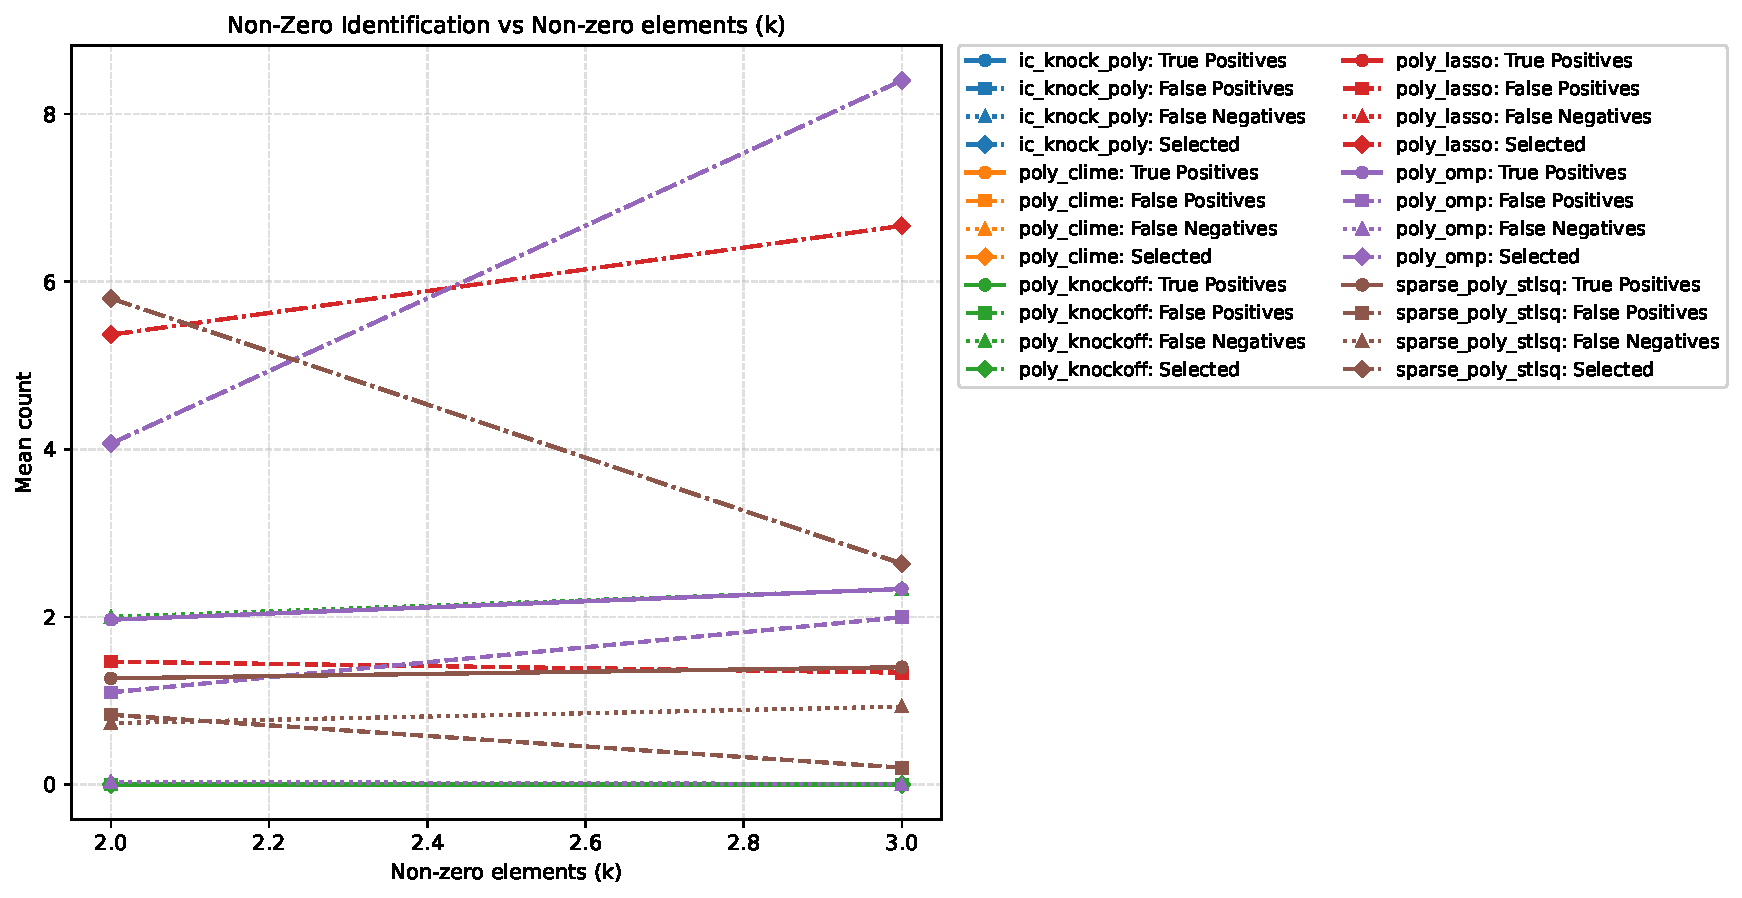
\includegraphics[width=0.9\textwidth]{figures/default_nonzero_identification_vs_k.pdf}
\caption{Nonzero Identification vs.\ k (default sweep)}
\label{fig:default_nonzero_identification_vs_k}
\end{figure}


\begin{figure}[htbp]
\centering
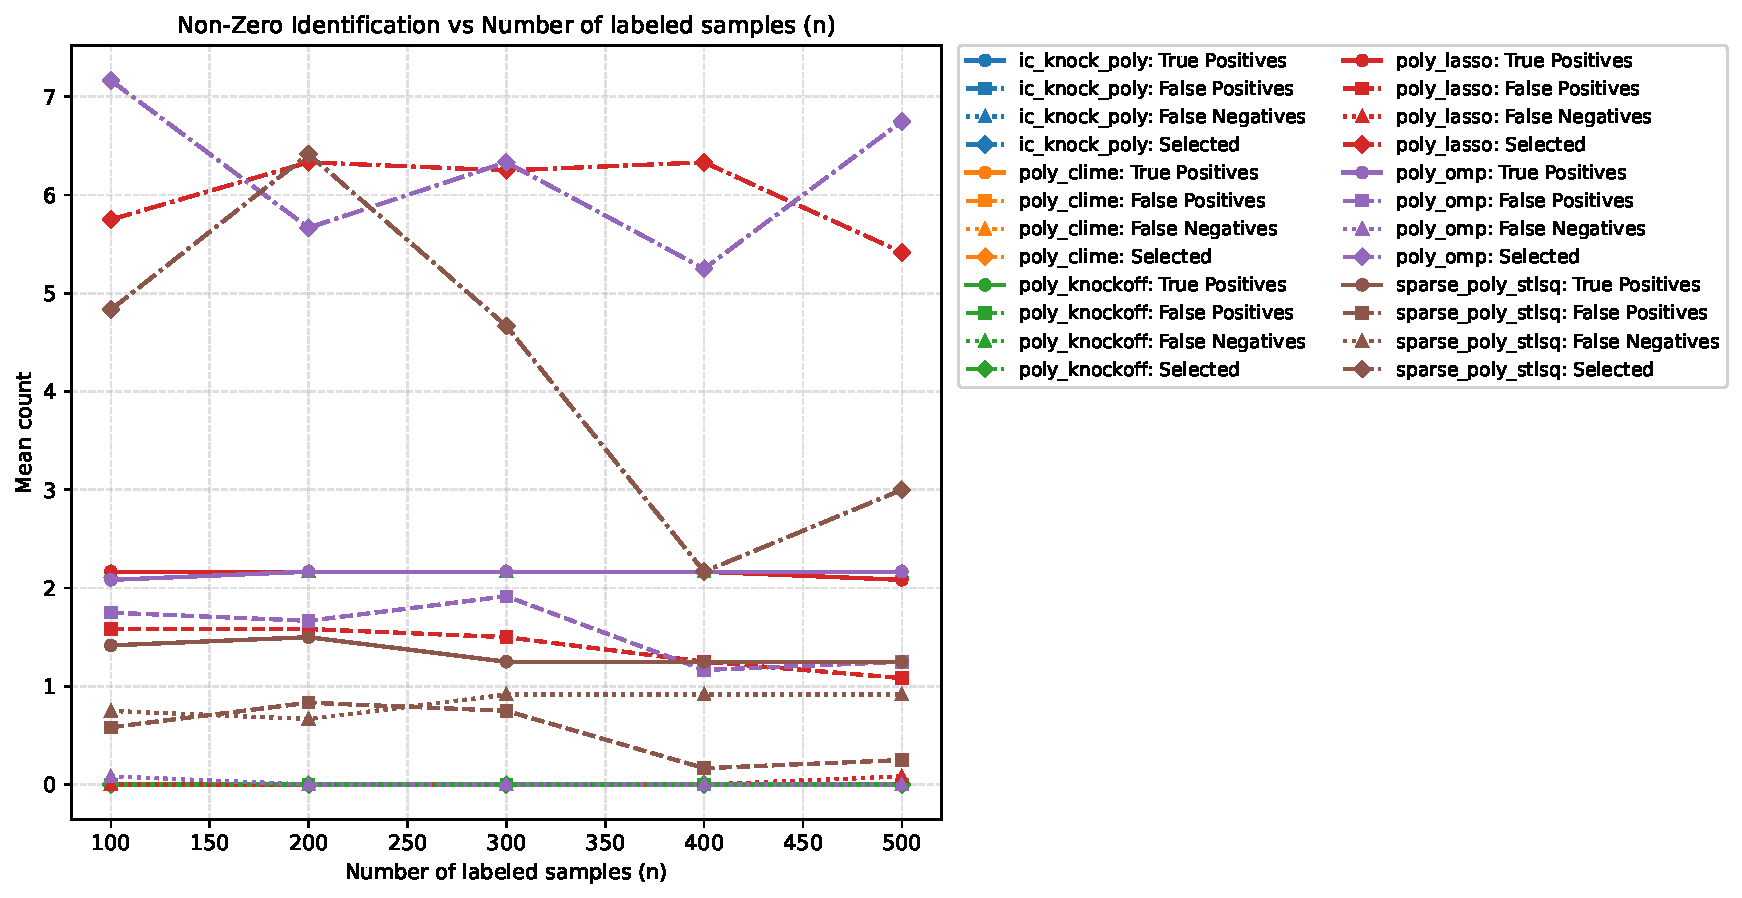
\includegraphics[width=0.9\textwidth]{figures/default_nonzero_identification_vs_n_labeled.pdf}
\caption{Nonzero Identification vs.\ n labeled (default sweep)}
\label{fig:default_nonzero_identification_vs_n_labeled}
\end{figure}


\begin{figure}[htbp]
\centering
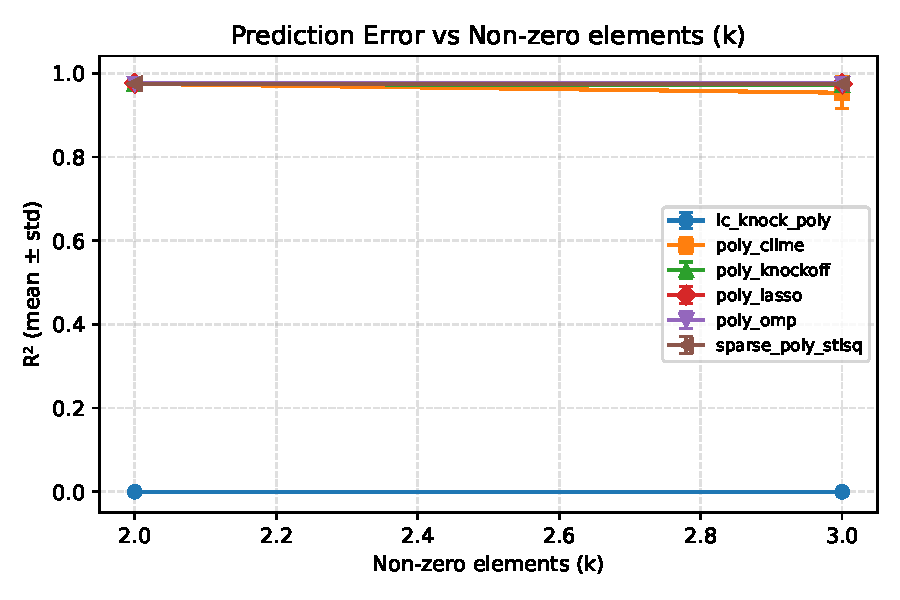
\includegraphics[width=0.9\textwidth]{figures/default_prediction_error_vs_k.pdf}
\caption{Prediction Error vs.\ k (default sweep)}
\label{fig:default_prediction_error_vs_k}
\end{figure}


\begin{figure}[htbp]
\centering
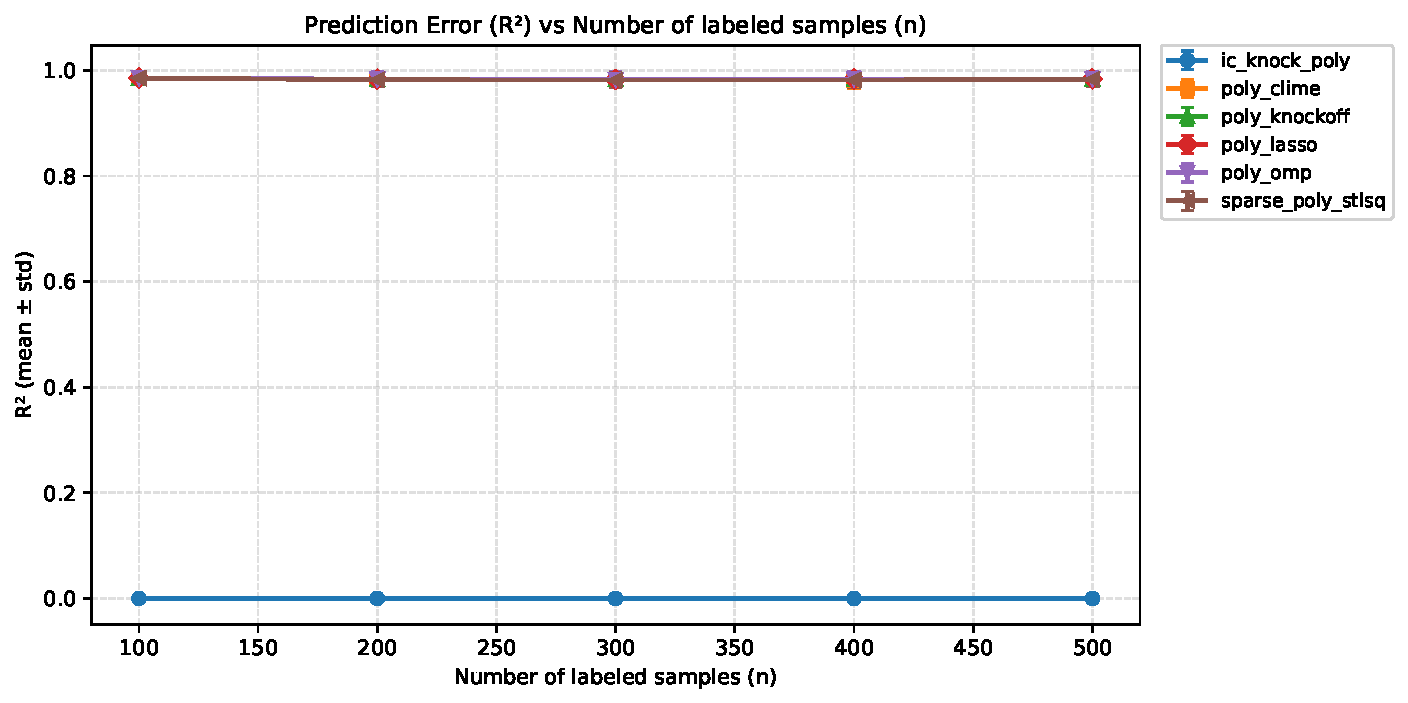
\includegraphics[width=0.9\textwidth]{figures/default_prediction_error_vs_n_labeled.pdf}
\caption{Prediction Error vs.\ n labeled (default sweep)}
\label{fig:default_prediction_error_vs_n_labeled}
\end{figure}


\begin{figure}[htbp]
\centering
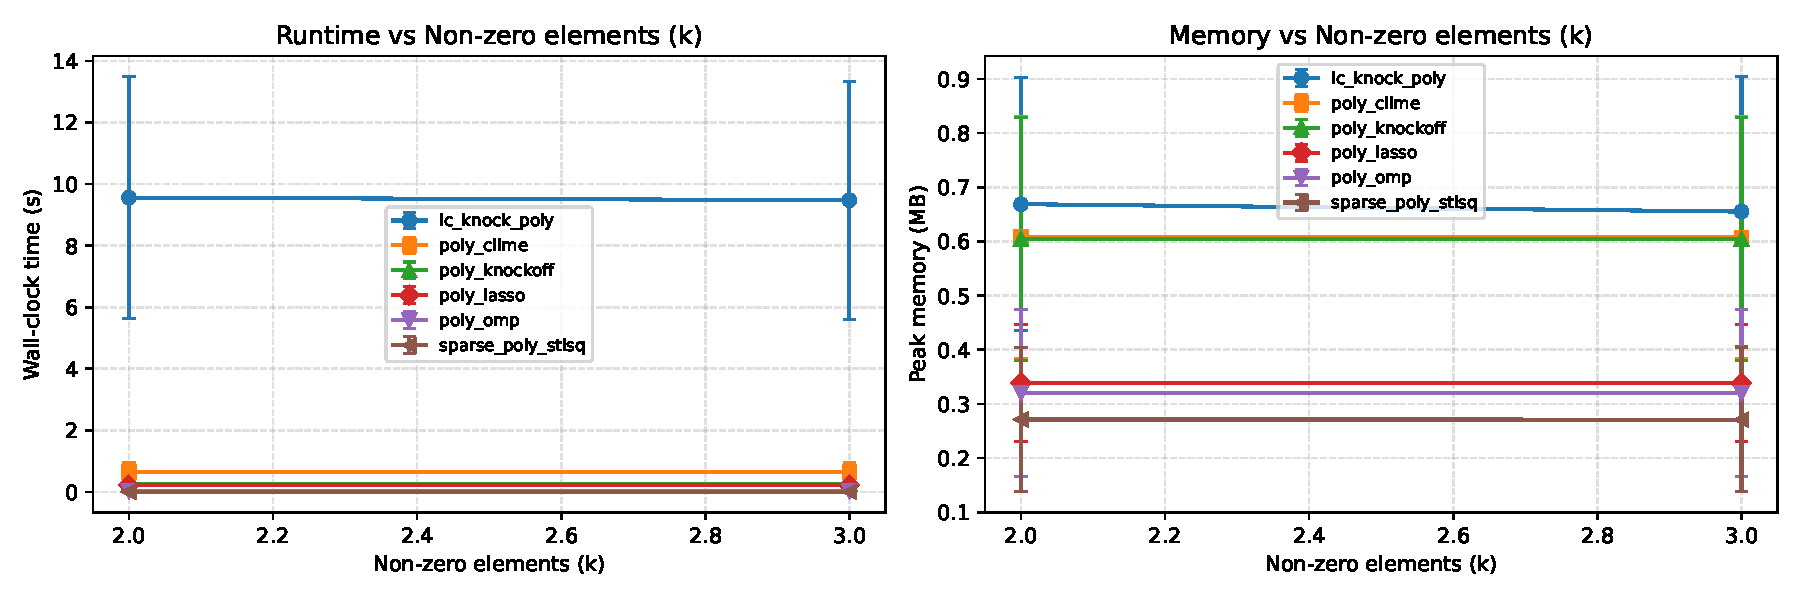
\includegraphics[width=0.9\textwidth]{figures/default_scalability_vs_k.pdf}
\caption{Scalability vs.\ k (default sweep)}
\label{fig:default_scalability_vs_k}
\end{figure}


\begin{figure}[htbp]
\centering
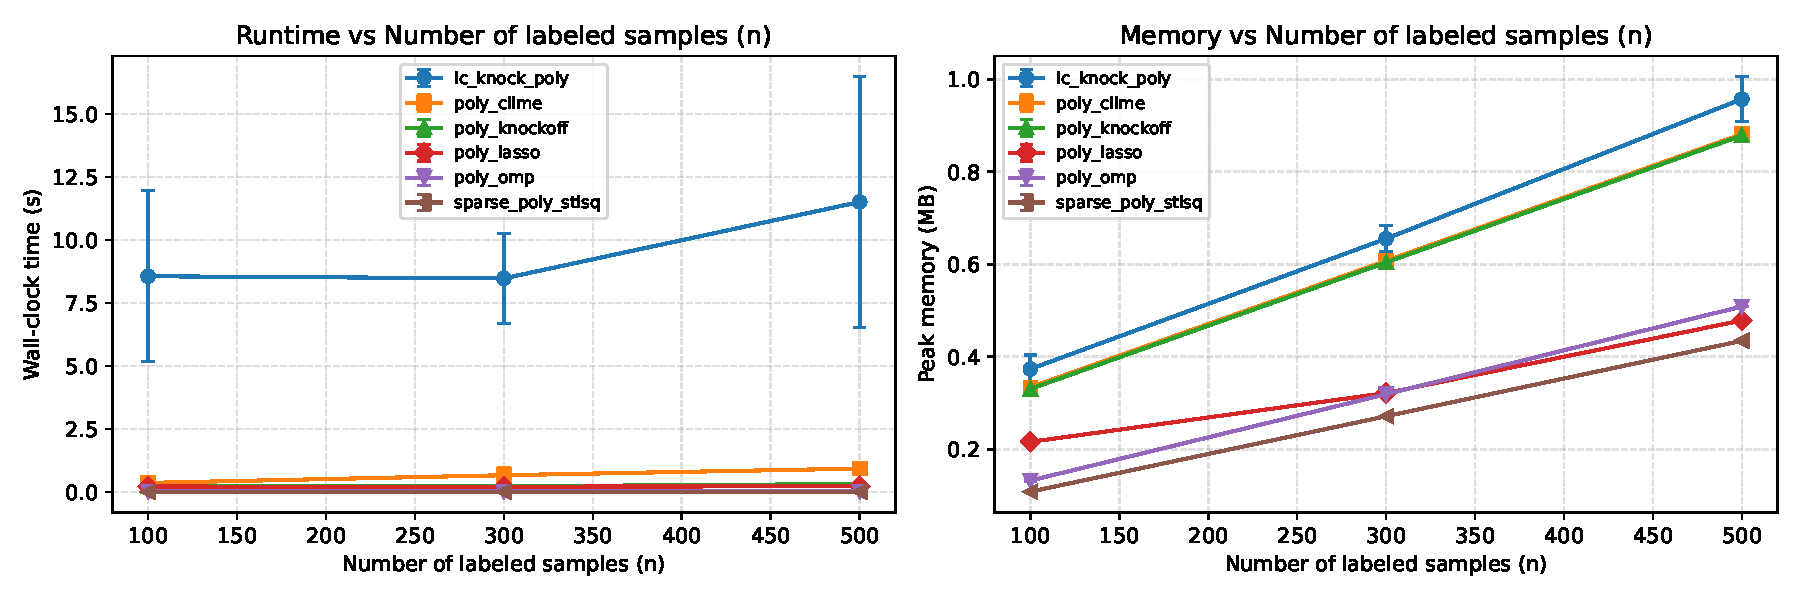
\includegraphics[width=0.9\textwidth]{figures/default_scalability_vs_n_labeled.pdf}
\caption{Scalability vs.\ n labeled (default sweep)}
\label{fig:default_scalability_vs_n_labeled}
\end{figure}


\begin{figure}[htbp]
\centering
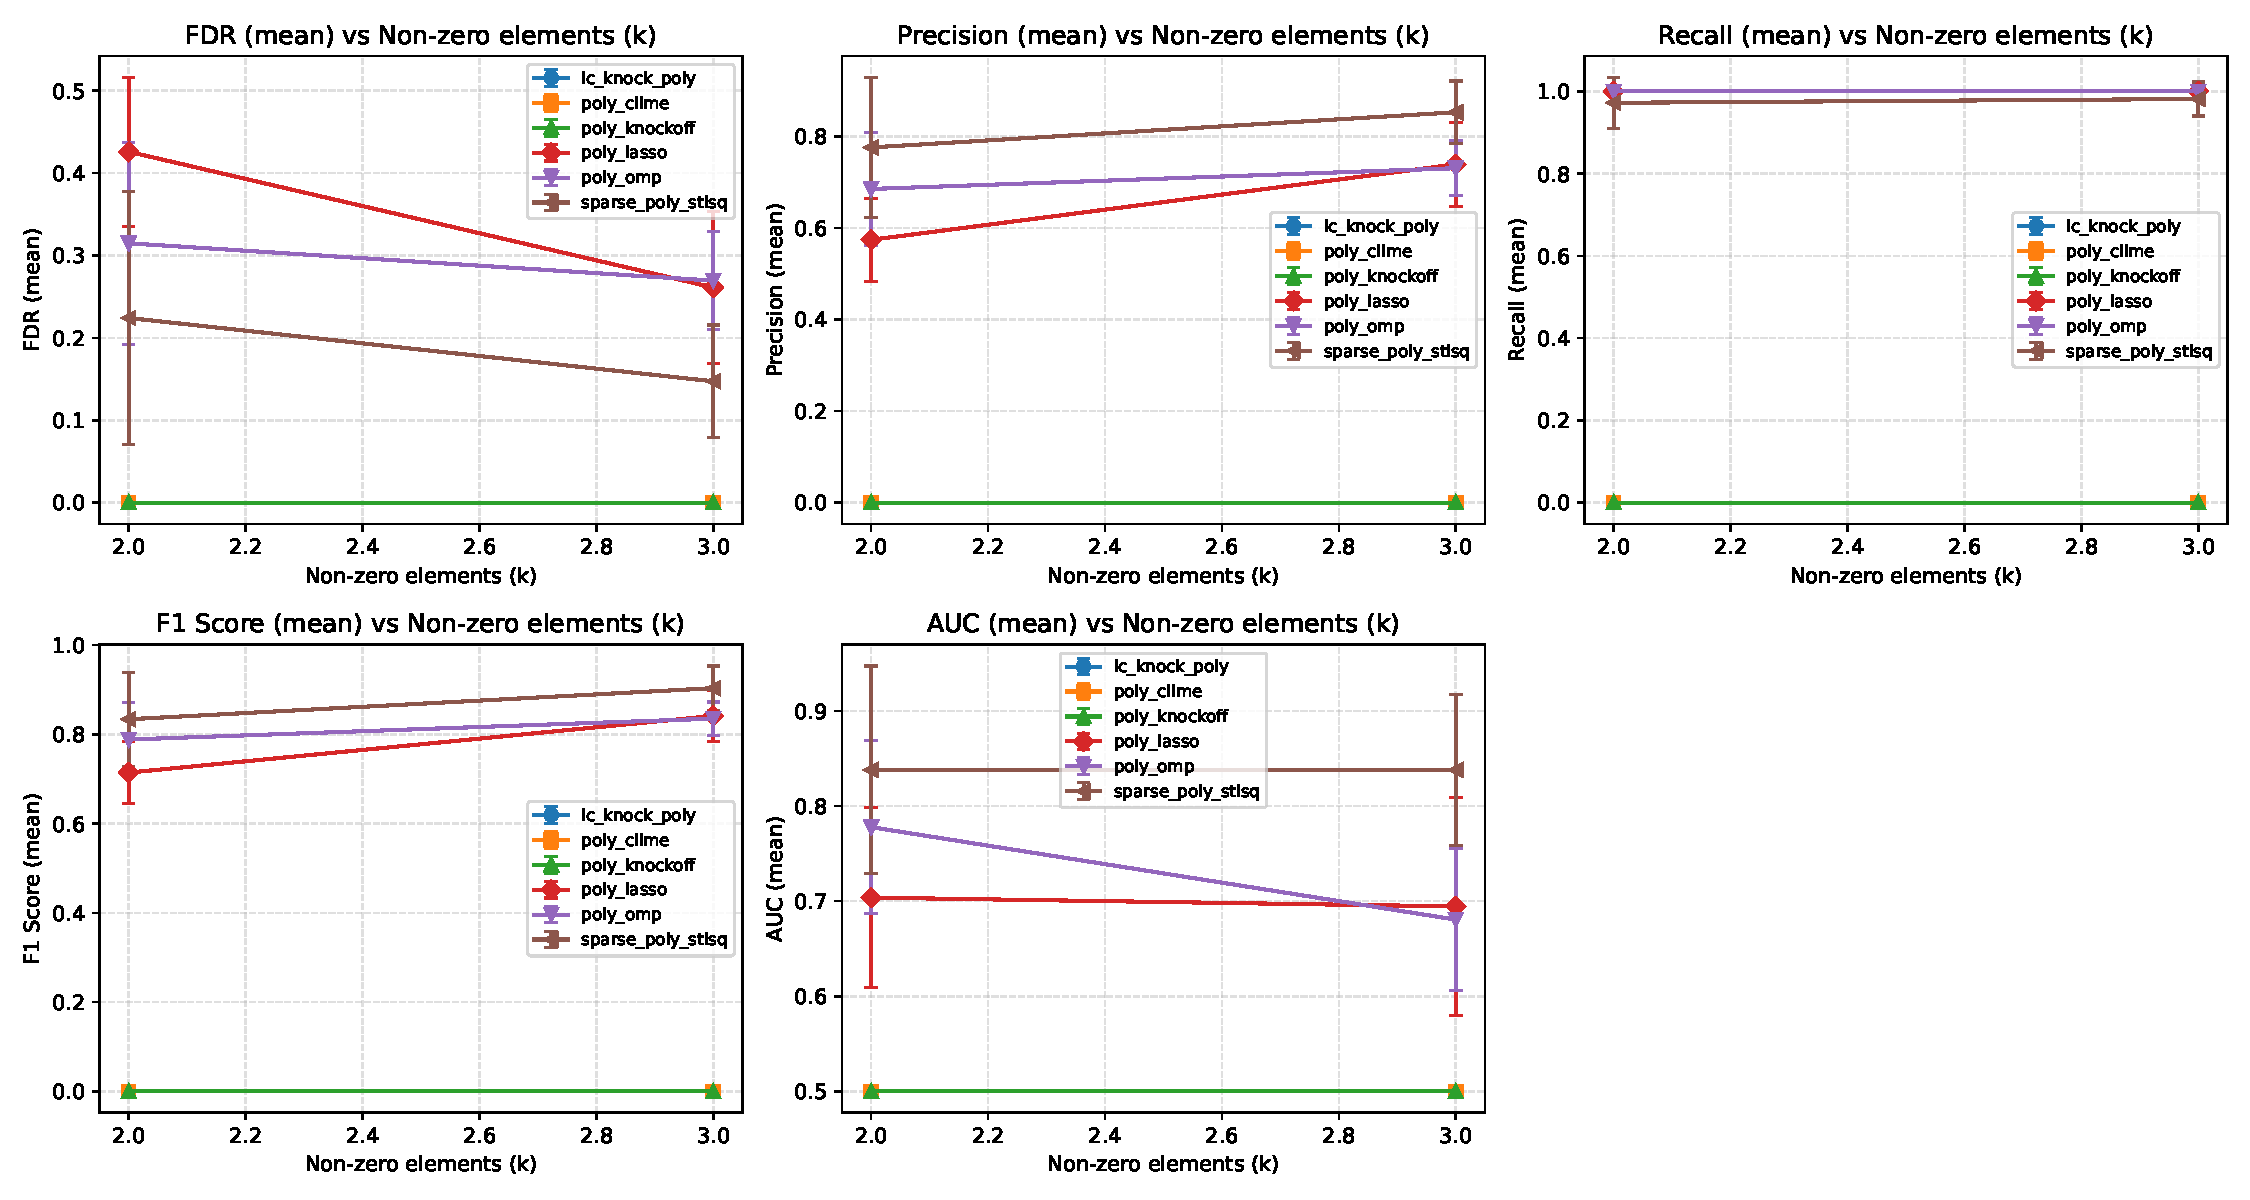
\includegraphics[width=0.9\textwidth]{figures/default_selection_metrics_vs_k.pdf}
\caption{Selection Metrics vs.\ k (default sweep)}
\label{fig:default_selection_metrics_vs_k}
\end{figure}


\begin{figure}[htbp]
\centering
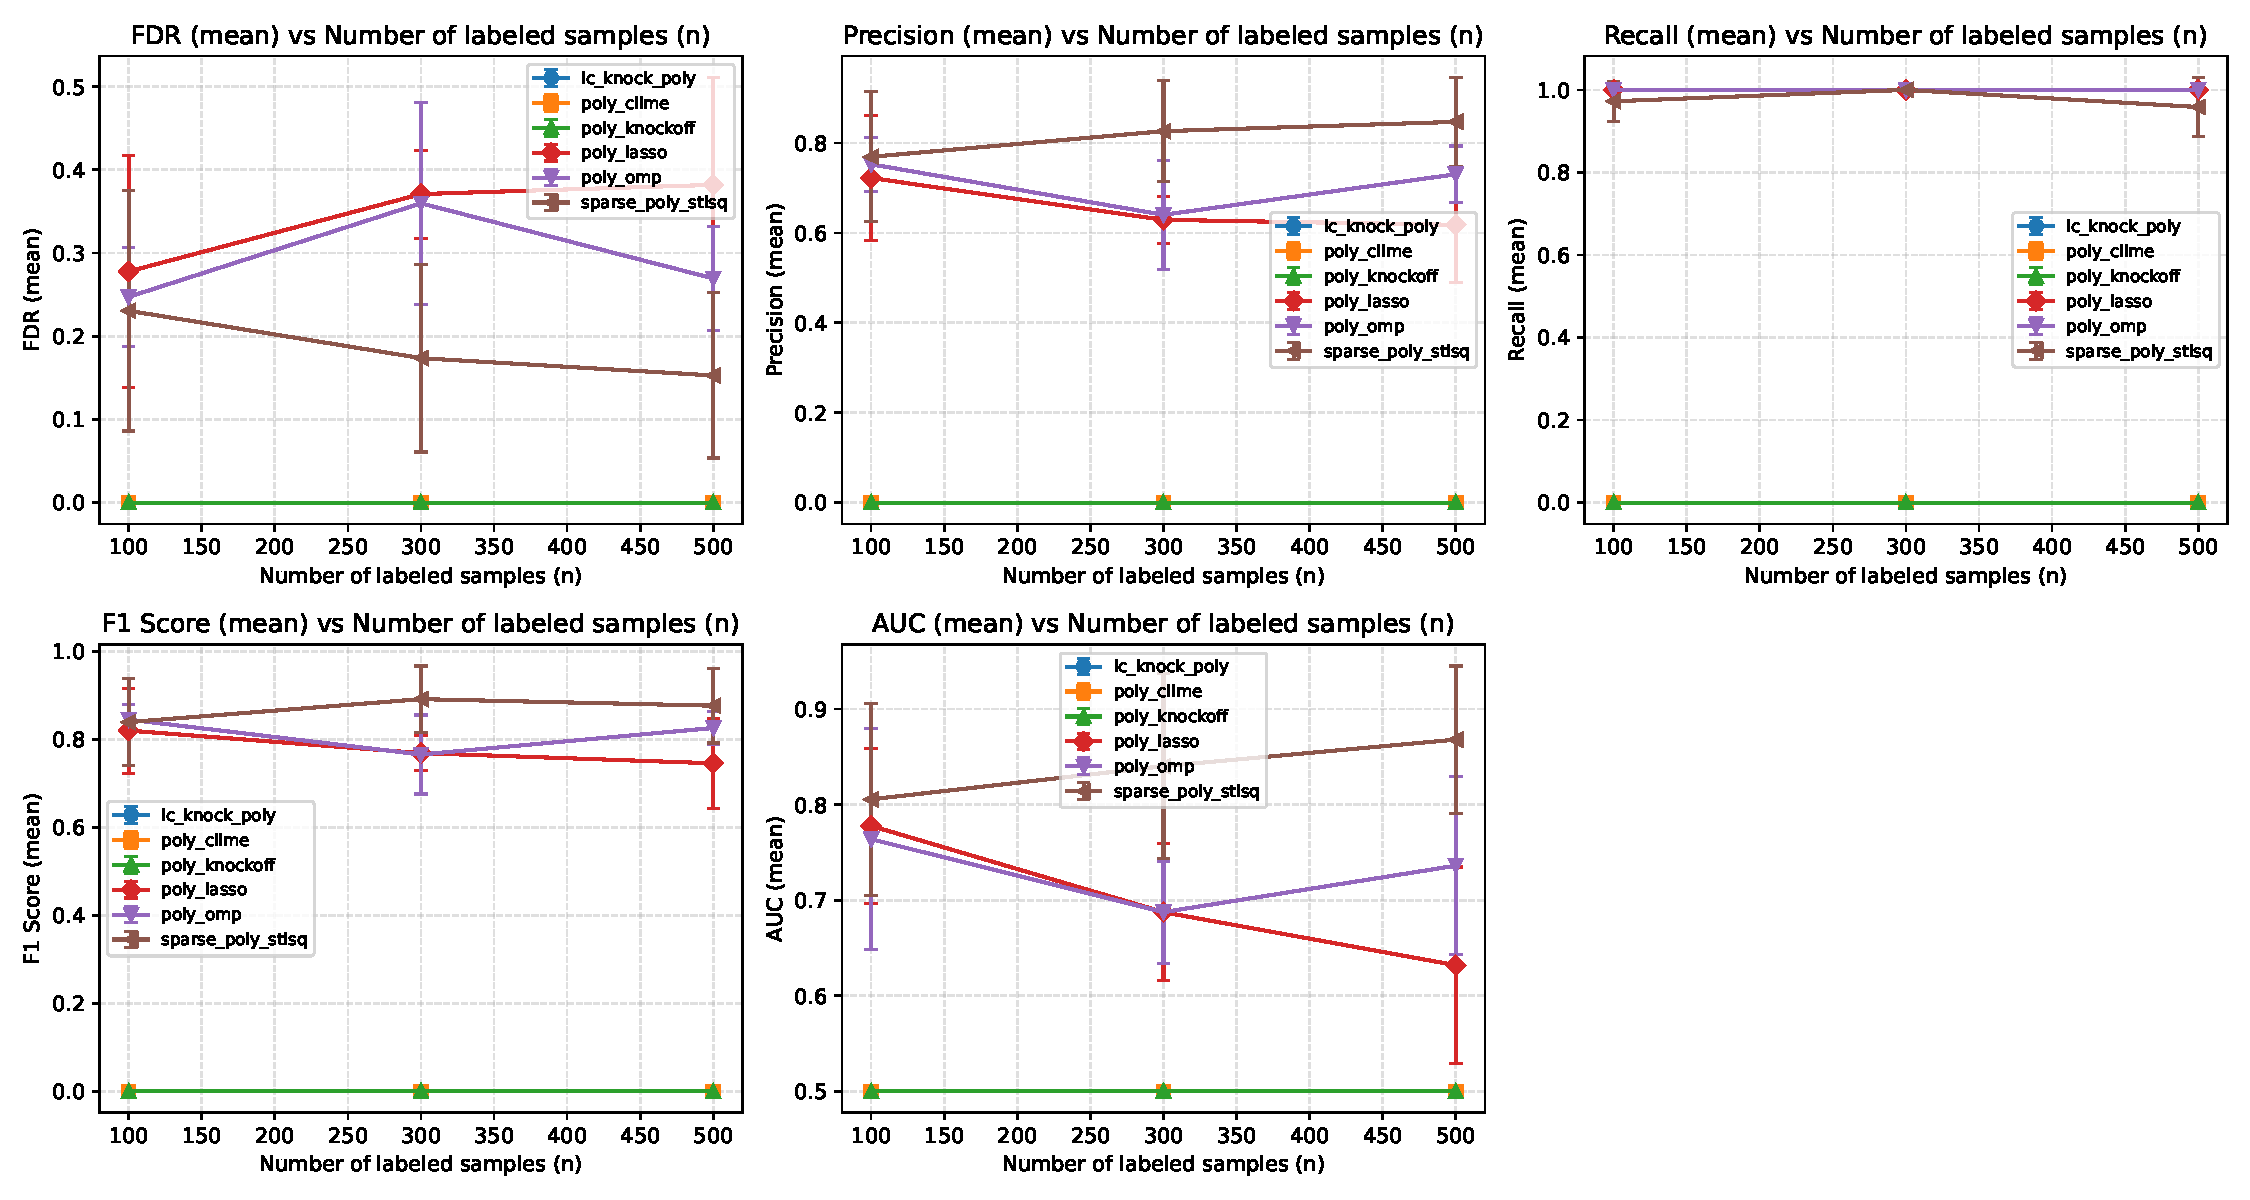
\includegraphics[width=0.9\textwidth]{figures/default_selection_metrics_vs_n_labeled.pdf}
\caption{Selection Metrics vs.\ n labeled (default sweep)}
\label{fig:default_selection_metrics_vs_n_labeled}
\end{figure}


% ===================================================================
\section{Degree\,$\times$\,Non-Zero Sweep}
\label{sec:degree_nonzero}

\subsection{Summary Table}

\Cref{tab:degree_nonzero} reports results for the degree-and-sparsity
sweep.


\begin{table}[htbp]
\centering
\caption{Degree $\times$ non-zero sweep results ($p=5$). Mean FDR, TPR, F1, AUC, R\textsuperscript{2}, and wall-clock time over completed trials.}
\label{tab:degree_nonzero}
\resizebox{\textwidth}{!}{%
\begin{tabular}{llccccccc}
\hline
\textbf{Config} & \textbf{Method} & \textbf{FDR} & \textbf{TPR} &
\textbf{F1} & \textbf{AUC} & \textbf{R\textsuperscript{2}} & \textbf{Time (s)} & \textbf{Trials} \\
\hline
  p5\_n100\_k2\_d2\_supervised & ic\_knock\_poly & 0.000 & 0.000 & 0.000 & 0.500 & 0.000 & 11.71 & 3 \\
  p5\_n100\_k2\_d2\_supervised & poly\_lasso & 0.444 & 1.000 & 0.711 & 0.722 & 0.979 & 0.22 & 3 \\
  p5\_n100\_k2\_d2\_supervised & poly\_omp & 0.222 & 1.000 & 0.867 & 0.889 & 0.980 & 0.03 & 3 \\
  p5\_n100\_k2\_d2\_supervised & poly\_clime & 0.000 & 0.000 & 0.000 & 0.500 & 0.979 & 0.41 & 3 \\
  p5\_n100\_k2\_d2\_supervised & poly\_knockoff & 0.000 & 0.000 & 0.000 & 0.500 & 0.979 & 0.23 & 3 \\
  p5\_n100\_k2\_d2\_supervised & sparse\_poly\_stlsq & 0.111 & 1.000 & 0.933 & 0.944 & 0.982 & 0.01 & 3 \\
  p5\_n300\_k2\_d2\_supervised & ic\_knock\_poly & 0.000 & 0.000 & 0.000 & 0.500 & 0.000 & 7.00 & 3 \\
  p5\_n300\_k2\_d2\_supervised & poly\_lasso & 0.444 & 1.000 & 0.711 & 0.722 & 0.974 & 0.21 & 3 \\
  p5\_n300\_k2\_d2\_supervised & poly\_omp & 0.444 & 1.000 & 0.711 & 0.722 & 0.974 & 0.03 & 3 \\
  p5\_n300\_k2\_d2\_supervised & poly\_clime & 0.000 & 0.000 & 0.000 & 0.500 & 0.973 & 0.99 & 3 \\
  p5\_n300\_k2\_d2\_supervised & poly\_knockoff & 0.000 & 0.000 & 0.000 & 0.500 & 0.973 & 0.22 & 3 \\
  p5\_n300\_k2\_d2\_supervised & sparse\_poly\_stlsq & 0.000 & 1.000 & 1.000 & 1.000 & 0.974 & 0.01 & 3 \\
  p5\_n100\_k3\_d2\_supervised & ic\_knock\_poly & 0.000 & 0.000 & 0.000 & 0.500 & 0.000 & 12.13 & 3 \\
  p5\_n100\_k3\_d2\_supervised & poly\_lasso & 0.083 & 1.000 & 0.952 & 0.917 & 0.979 & 0.23 & 3 \\
  p5\_n100\_k3\_d2\_supervised & poly\_omp & 0.217 & 1.000 & 0.869 & 0.750 & 0.983 & 0.03 & 3 \\
  p5\_n100\_k3\_d2\_supervised & poly\_clime & 0.000 & 0.000 & 0.000 & 0.500 & 0.869 & 0.40 & 3 \\
  p5\_n100\_k3\_d2\_supervised & poly\_knockoff & 0.000 & 0.000 & 0.000 & 0.500 & 0.977 & 0.24 & 3 \\
  p5\_n100\_k3\_d2\_supervised & sparse\_poly\_stlsq & 0.167 & 1.000 & 0.905 & 0.833 & 0.981 & 0.01 & 3 \\
  p5\_n300\_k3\_d2\_supervised & ic\_knock\_poly & 0.000 & 0.000 & 0.000 & 0.500 & 0.000 & 6.61 & 3 \\
  p5\_n300\_k3\_d2\_supervised & poly\_lasso & 0.350 & 1.000 & 0.786 & 0.583 & 0.972 & 0.21 & 3 \\
  p5\_n300\_k3\_d2\_supervised & poly\_omp & 0.267 & 1.000 & 0.833 & 0.667 & 0.971 & 0.03 & 3 \\
  p5\_n300\_k3\_d2\_supervised & poly\_clime & 0.000 & 0.000 & 0.000 & 0.500 & 0.971 & 1.00 & 3 \\
  p5\_n300\_k3\_d2\_supervised & poly\_knockoff & 0.000 & 0.000 & 0.000 & 0.500 & 0.970 & 0.23 & 3 \\
  p5\_n300\_k3\_d2\_supervised & sparse\_poly\_stlsq & 0.217 & 1.000 & 0.869 & 0.750 & 0.973 & 0.01 & 3 \\
  p5\_n100\_k4\_d2\_supervised & ic\_knock\_poly & 0.000 & 0.000 & 0.000 & 0.500 & 0.000 & 11.65 & 3 \\
  p5\_n100\_k4\_d2\_supervised & poly\_lasso & 0.200 & 1.000 & 0.889 & 0.500 & 0.990 & 0.21 & 3 \\
  p5\_n100\_k4\_d2\_supervised & poly\_omp & 0.133 & 1.000 & 0.926 & 0.667 & 0.991 & 0.03 & 3 \\
  p5\_n100\_k4\_d2\_supervised & poly\_clime & 0.000 & 0.000 & 0.000 & 0.500 & 0.946 & 0.38 & 3 \\
  p5\_n100\_k4\_d2\_supervised & poly\_knockoff & 0.000 & 0.000 & 0.000 & 0.500 & 0.973 & 0.23 & 3 \\
  p5\_n100\_k4\_d2\_supervised & sparse\_poly\_stlsq & 0.133 & 1.000 & 0.926 & 0.667 & 0.991 & 0.01 & 3 \\
  p5\_n300\_k4\_d2\_supervised & ic\_knock\_poly & 0.000 & 0.000 & 0.000 & 0.500 & 0.000 & 6.58 & 3 \\
  p5\_n300\_k4\_d2\_supervised & poly\_lasso & 0.200 & 1.000 & 0.889 & 0.500 & 0.988 & 0.21 & 3 \\
  p5\_n300\_k4\_d2\_supervised & poly\_omp & 0.200 & 1.000 & 0.889 & 0.500 & 0.988 & 0.03 & 3 \\
  p5\_n300\_k4\_d2\_supervised & poly\_clime & 0.000 & 0.333 & 0.333 & 0.667 & 0.987 & 0.99 & 3 \\
  p5\_n300\_k4\_d2\_supervised & poly\_knockoff & 0.000 & 0.333 & 0.333 & 0.667 & 0.988 & 0.22 & 3 \\
  p5\_n300\_k4\_d2\_supervised & sparse\_poly\_stlsq & 0.067 & 1.000 & 0.963 & 0.833 & 0.988 & 0.01 & 3 \\
  p5\_n100\_k2\_d3\_supervised & ic\_knock\_poly & 0.000 & 0.000 & 0.000 & 0.500 & 0.000 & 11.67 & 3 \\
  p5\_n100\_k2\_d3\_supervised & poly\_lasso & 0.511 & 1.000 & 0.648 & 0.611 & 0.981 & 0.21 & 3 \\
  p5\_n100\_k2\_d3\_supervised & poly\_omp & 0.478 & 1.000 & 0.679 & 0.667 & 0.980 & 0.03 & 3 \\
  p5\_n100\_k2\_d3\_supervised & poly\_clime & 0.000 & 0.000 & 0.000 & 0.500 & 0.979 & 0.40 & 3 \\
  p5\_n100\_k2\_d3\_supervised & poly\_knockoff & 0.000 & 0.000 & 0.000 & 0.500 & 0.979 & 0.23 & 3 \\
  p5\_n100\_k2\_d3\_supervised & sparse\_poly\_stlsq & 0.667 & 0.167 & 0.222 & 0.417 & 0.339 & 0.01 & 3 \\
  p5\_n300\_k2\_d3\_supervised & ic\_knock\_poly & 0.000 & 0.000 & 0.000 & 0.500 & 0.000 & 6.80 & 3 \\
  p5\_n300\_k2\_d3\_supervised & poly\_lasso & 0.444 & 1.000 & 0.711 & 0.722 & 0.974 & 0.22 & 3 \\
  p5\_n300\_k2\_d3\_supervised & poly\_omp & 0.500 & 1.000 & 0.667 & 0.667 & 0.974 & 0.03 & 3 \\
  p5\_n300\_k2\_d3\_supervised & poly\_clime & 0.000 & 0.000 & 0.000 & 0.500 & 0.973 & 1.07 & 3 \\
  p5\_n300\_k2\_d3\_supervised & poly\_knockoff & 0.000 & 0.000 & 0.000 & 0.500 & 0.973 & 0.31 & 3 \\
  p5\_n300\_k2\_d3\_supervised & sparse\_poly\_stlsq & 0.722 & 0.333 & 0.300 & 0.444 & 0.642 & 0.01 & 3 \\
  p5\_n100\_k3\_d3\_supervised & ic\_knock\_poly & 0.000 & 0.000 & 0.000 & 0.500 & 0.000 & 11.83 & 3 \\
  p5\_n100\_k3\_d3\_supervised & poly\_lasso & 0.167 & 1.000 & 0.905 & 0.833 & 0.979 & 0.23 & 3 \\
  p5\_n100\_k3\_d3\_supervised & poly\_omp & 0.133 & 1.000 & 0.917 & 0.833 & 0.983 & 0.03 & 3 \\
  p5\_n100\_k3\_d3\_supervised & poly\_clime & 0.000 & 0.000 & 0.000 & 0.500 & 0.865 & 0.41 & 3 \\
  p5\_n100\_k3\_d3\_supervised & poly\_knockoff & 0.000 & 0.000 & 0.000 & 0.500 & 0.976 & 0.25 & 3 \\
  p5\_n100\_k3\_d3\_supervised & sparse\_poly\_stlsq & 0.194 & 0.778 & 0.775 & 0.722 & 0.802 & 0.01 & 3 \\
  p5\_n300\_k3\_d3\_supervised & ic\_knock\_poly & 0.000 & 0.000 & 0.000 & 0.500 & 0.000 & 6.75 & 3 \\
  p5\_n300\_k3\_d3\_supervised & poly\_lasso & 0.217 & 1.000 & 0.869 & 0.750 & 0.972 & 0.23 & 3 \\
  p5\_n300\_k3\_d3\_supervised & poly\_omp & 0.267 & 1.000 & 0.833 & 0.667 & 0.973 & 0.04 & 3 \\
  p5\_n300\_k3\_d3\_supervised & poly\_clime & 0.000 & 0.000 & 0.000 & 0.500 & 0.971 & 1.09 & 3 \\
  p5\_n300\_k3\_d3\_supervised & poly\_knockoff & 0.000 & 0.000 & 0.000 & 0.500 & 0.970 & 0.32 & 3 \\
  p5\_n300\_k3\_d3\_supervised & sparse\_poly\_stlsq & 0.467 & 0.667 & 0.583 & 0.417 & 0.903 & 0.01 & 3 \\
  p5\_n100\_k4\_d3\_supervised & ic\_knock\_poly & 0.000 & 0.000 & 0.000 & 0.500 & 0.000 & 11.69 & 3 \\
  p5\_n100\_k4\_d3\_supervised & poly\_lasso & 0.200 & 1.000 & 0.889 & 0.500 & 0.990 & 0.22 & 3 \\
  p5\_n100\_k4\_d3\_supervised & poly\_omp & 0.133 & 1.000 & 0.926 & 0.667 & 0.990 & 0.03 & 3 \\
  p5\_n100\_k4\_d3\_supervised & poly\_clime & 0.000 & 0.000 & 0.000 & 0.500 & 0.953 & 0.39 & 3 \\
  p5\_n100\_k4\_d3\_supervised & poly\_knockoff & 0.000 & 0.000 & 0.000 & 0.500 & 0.974 & 0.23 & 3 \\
  p5\_n100\_k4\_d3\_supervised & sparse\_poly\_stlsq & 0.000 & 0.667 & 0.778 & 0.833 & 0.757 & 0.01 & 3 \\
  p5\_n300\_k4\_d3\_supervised & ic\_knock\_poly & 0.000 & 0.000 & 0.000 & 0.500 & 0.000 & 6.76 & 3 \\
  p5\_n300\_k4\_d3\_supervised & poly\_lasso & 0.200 & 1.000 & 0.889 & 0.500 & 0.988 & 0.23 & 3 \\
  p5\_n300\_k4\_d3\_supervised & poly\_omp & 0.200 & 1.000 & 0.889 & 0.500 & 0.988 & 0.04 & 3 \\
  p5\_n300\_k4\_d3\_supervised & poly\_clime & 0.067 & 0.667 & 0.630 & 0.667 & 0.988 & 1.12 & 3 \\
  p5\_n300\_k4\_d3\_supervised & poly\_knockoff & 0.000 & 0.667 & 0.667 & 0.833 & 0.988 & 0.32 & 3 \\
  p5\_n300\_k4\_d3\_supervised & sparse\_poly\_stlsq & 0.000 & 0.667 & 0.752 & 0.833 & 0.681 & 0.02 & 3 \\
\hline
\end{tabular}%
}
\end{table}


\subsection{Figures}


\begin{figure}[htbp]
\centering
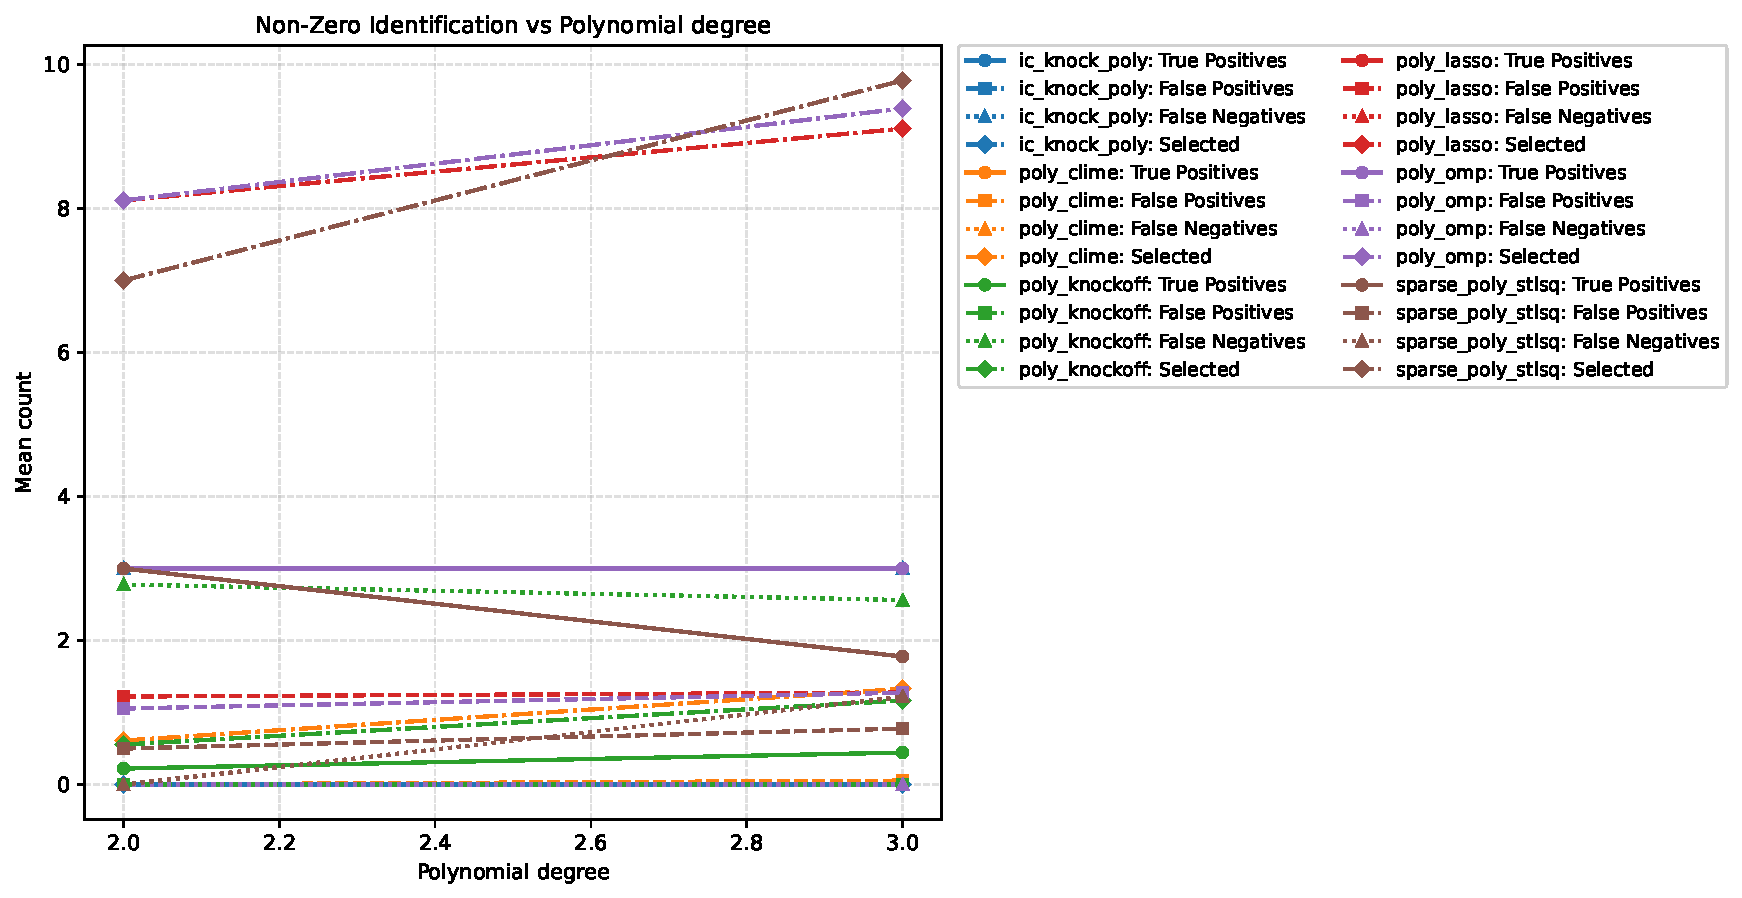
\includegraphics[width=0.9\textwidth]{figures/degree_nonzero_nonzero_identification_vs_degree.pdf}
\caption{Nonzero Identification vs.\ degree (degree nonzero sweep)}
\label{fig:degree_nonzero_nonzero_identification_vs_degree}
\end{figure}


\begin{figure}[htbp]
\centering
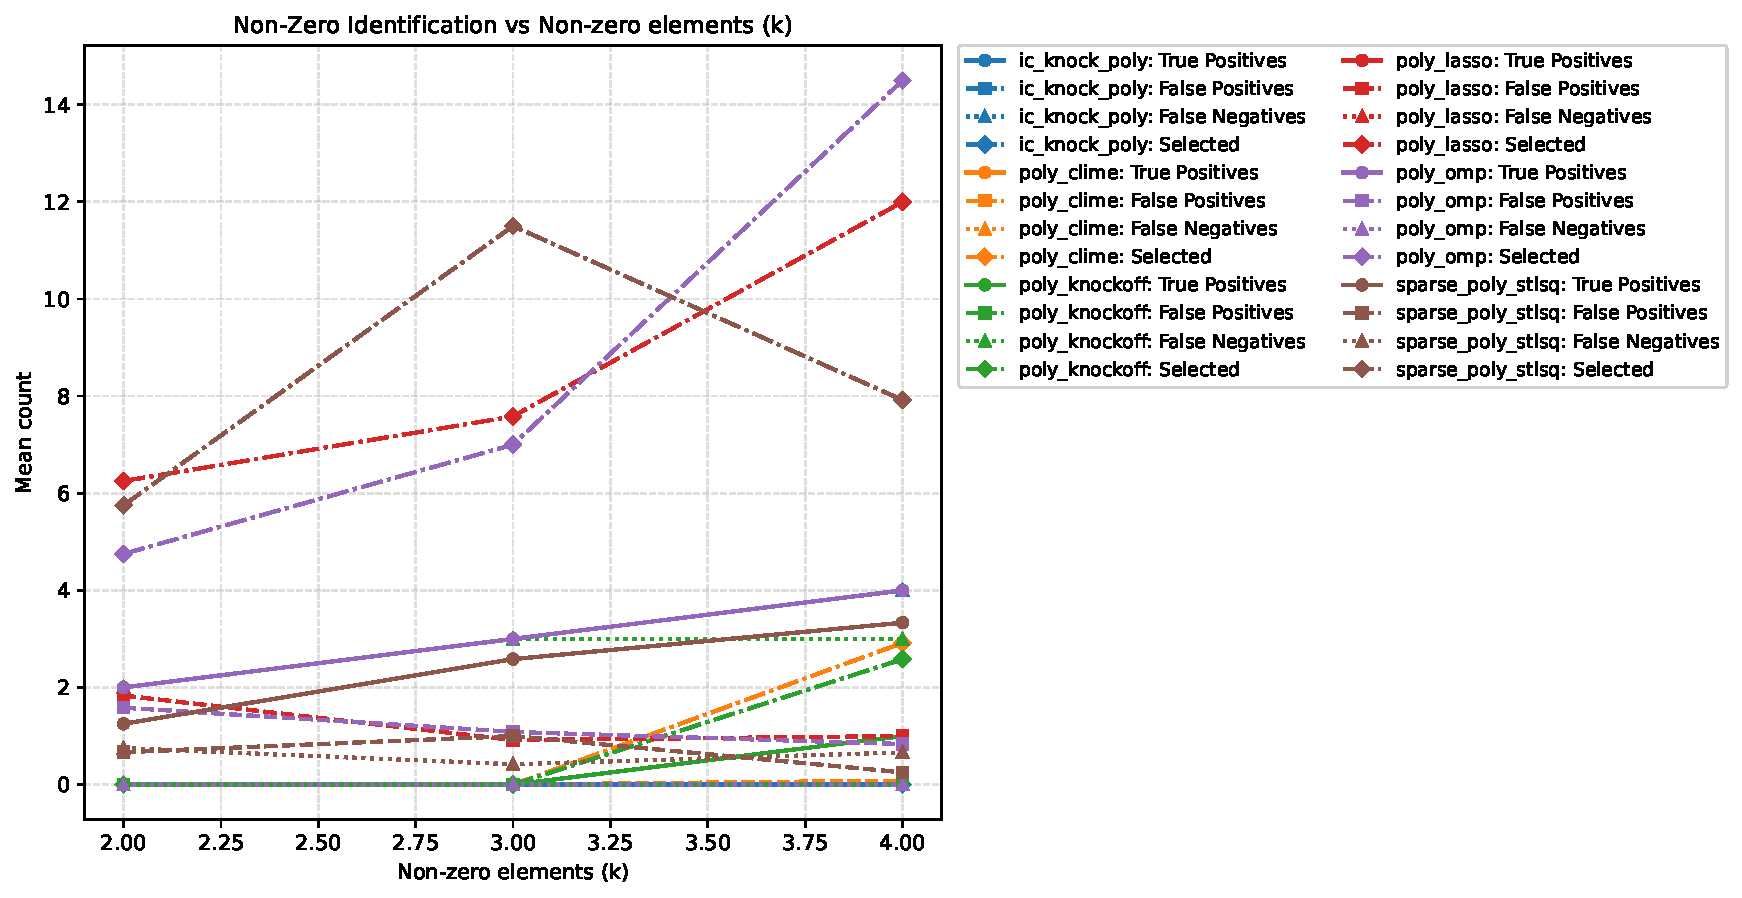
\includegraphics[width=0.9\textwidth]{figures/degree_nonzero_nonzero_identification_vs_k.pdf}
\caption{Nonzero Identification vs.\ k (degree nonzero sweep)}
\label{fig:degree_nonzero_nonzero_identification_vs_k}
\end{figure}


\begin{figure}[htbp]
\centering
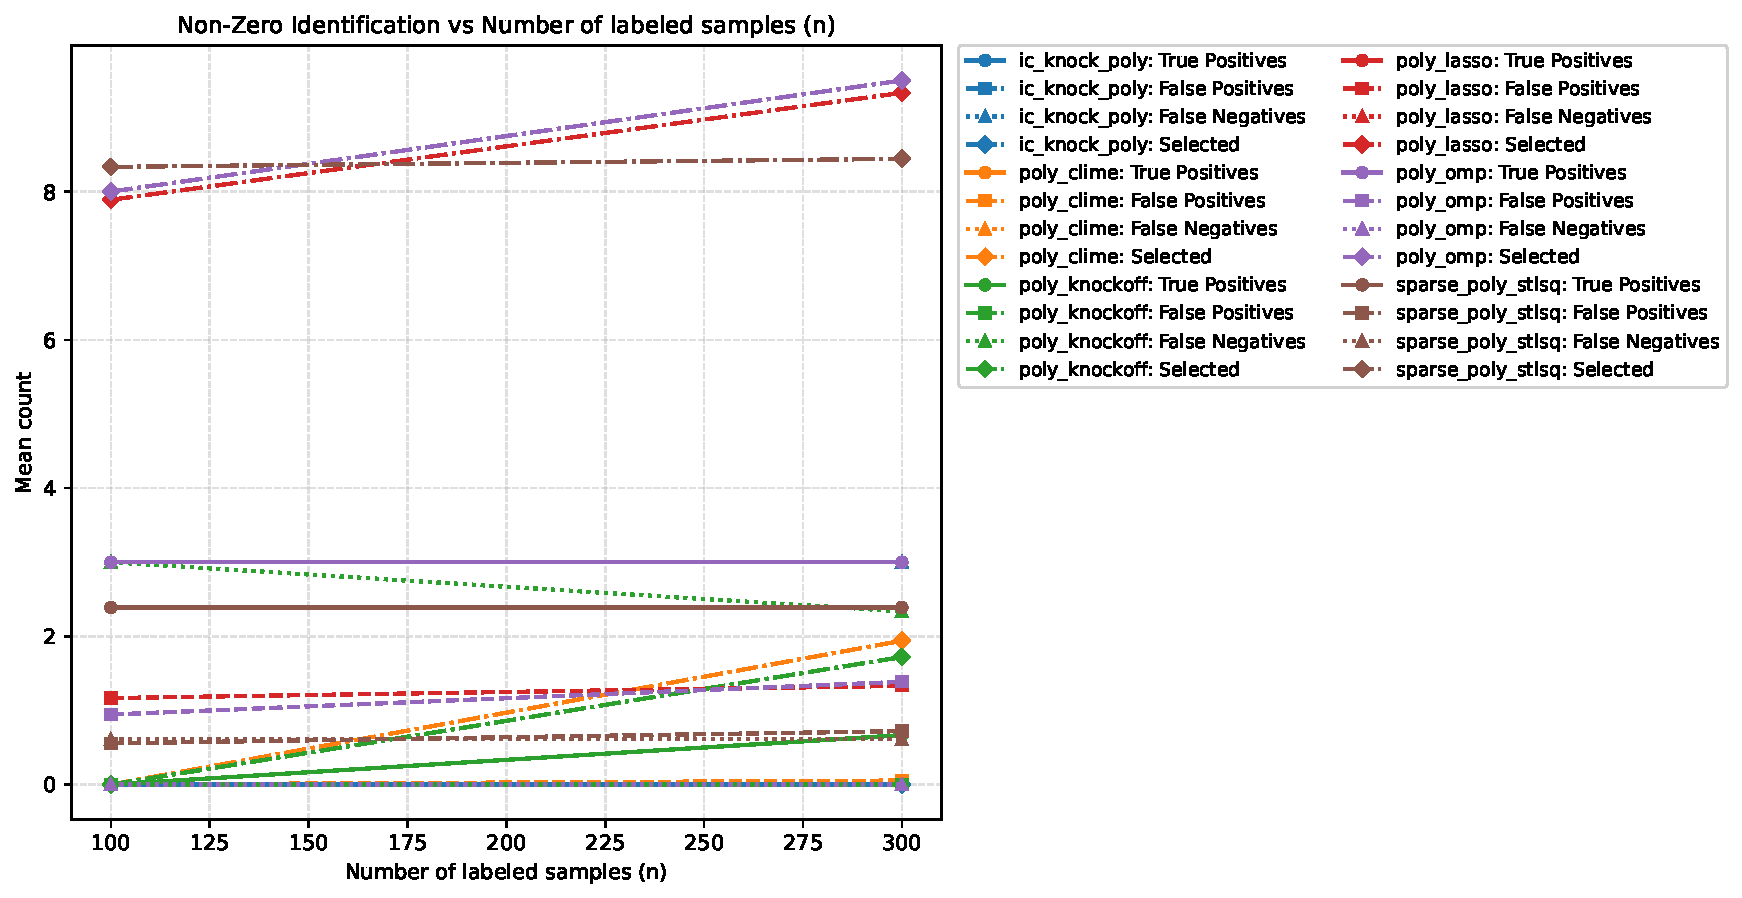
\includegraphics[width=0.9\textwidth]{figures/degree_nonzero_nonzero_identification_vs_n_labeled.pdf}
\caption{Nonzero Identification vs.\ n labeled (degree nonzero sweep)}
\label{fig:degree_nonzero_nonzero_identification_vs_n_labeled}
\end{figure}


\begin{figure}[htbp]
\centering
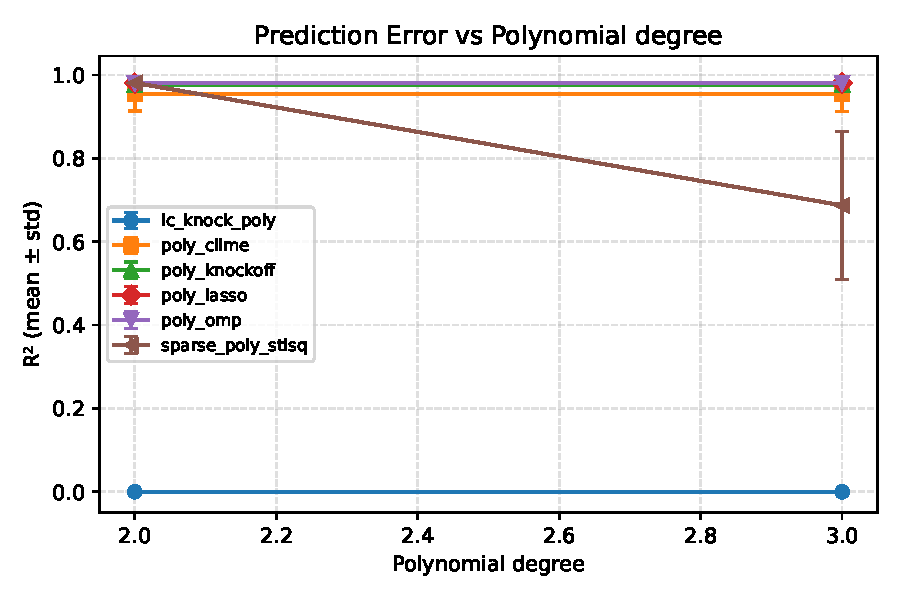
\includegraphics[width=0.9\textwidth]{figures/degree_nonzero_prediction_error_vs_degree.pdf}
\caption{Prediction Error vs.\ degree (degree nonzero sweep)}
\label{fig:degree_nonzero_prediction_error_vs_degree}
\end{figure}


\begin{figure}[htbp]
\centering
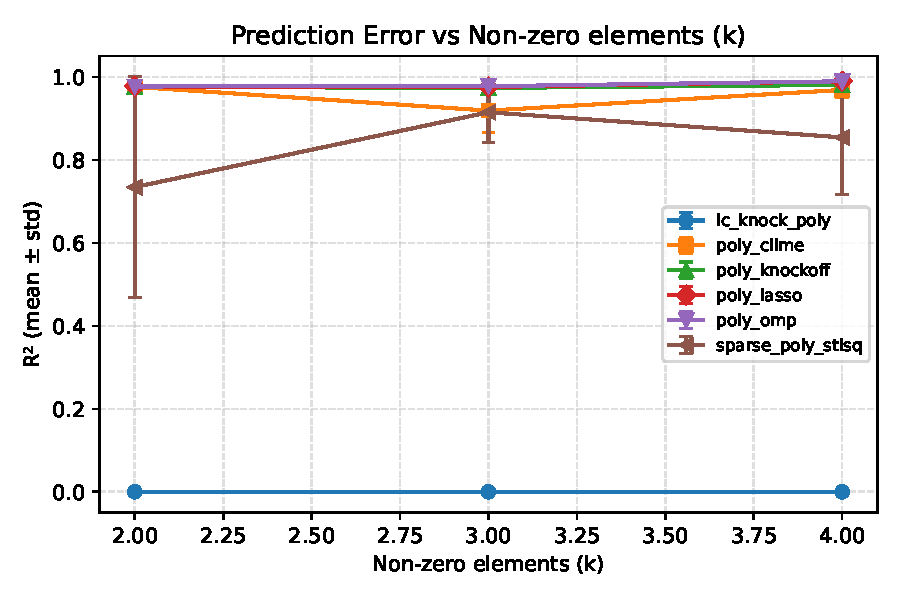
\includegraphics[width=0.9\textwidth]{figures/degree_nonzero_prediction_error_vs_k.pdf}
\caption{Prediction Error vs.\ k (degree nonzero sweep)}
\label{fig:degree_nonzero_prediction_error_vs_k}
\end{figure}


\begin{figure}[htbp]
\centering
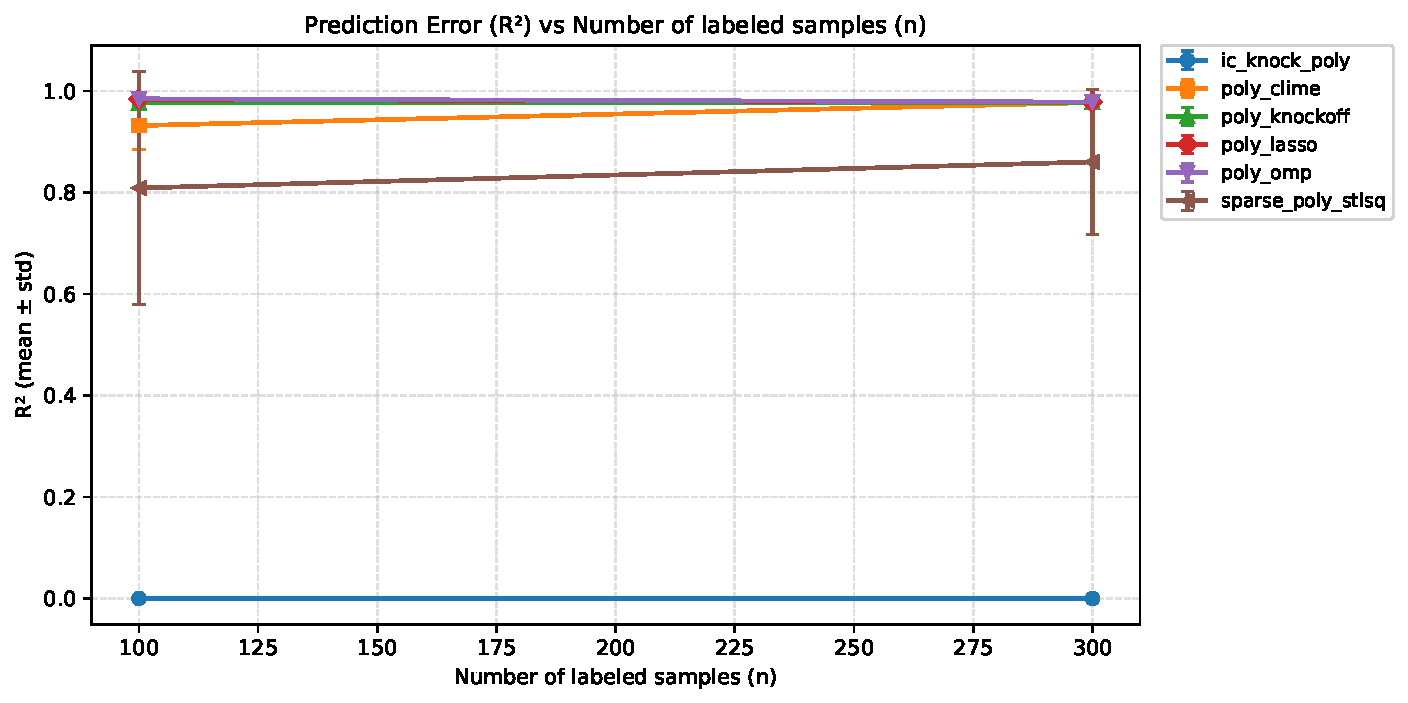
\includegraphics[width=0.9\textwidth]{figures/degree_nonzero_prediction_error_vs_n_labeled.pdf}
\caption{Prediction Error vs.\ n labeled (degree nonzero sweep)}
\label{fig:degree_nonzero_prediction_error_vs_n_labeled}
\end{figure}


\begin{figure}[htbp]
\centering
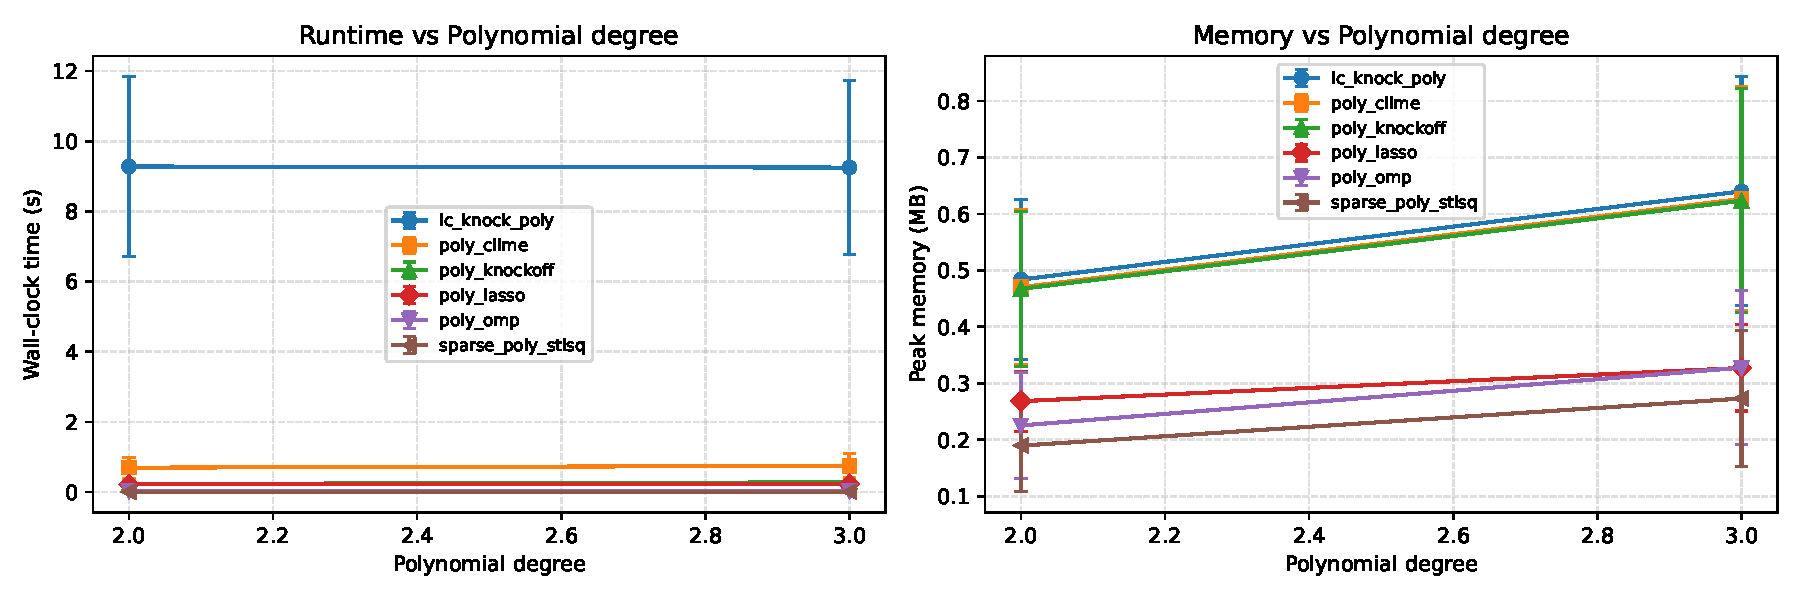
\includegraphics[width=0.9\textwidth]{figures/degree_nonzero_scalability_vs_degree.pdf}
\caption{Scalability vs.\ degree (degree nonzero sweep)}
\label{fig:degree_nonzero_scalability_vs_degree}
\end{figure}


\begin{figure}[htbp]
\centering
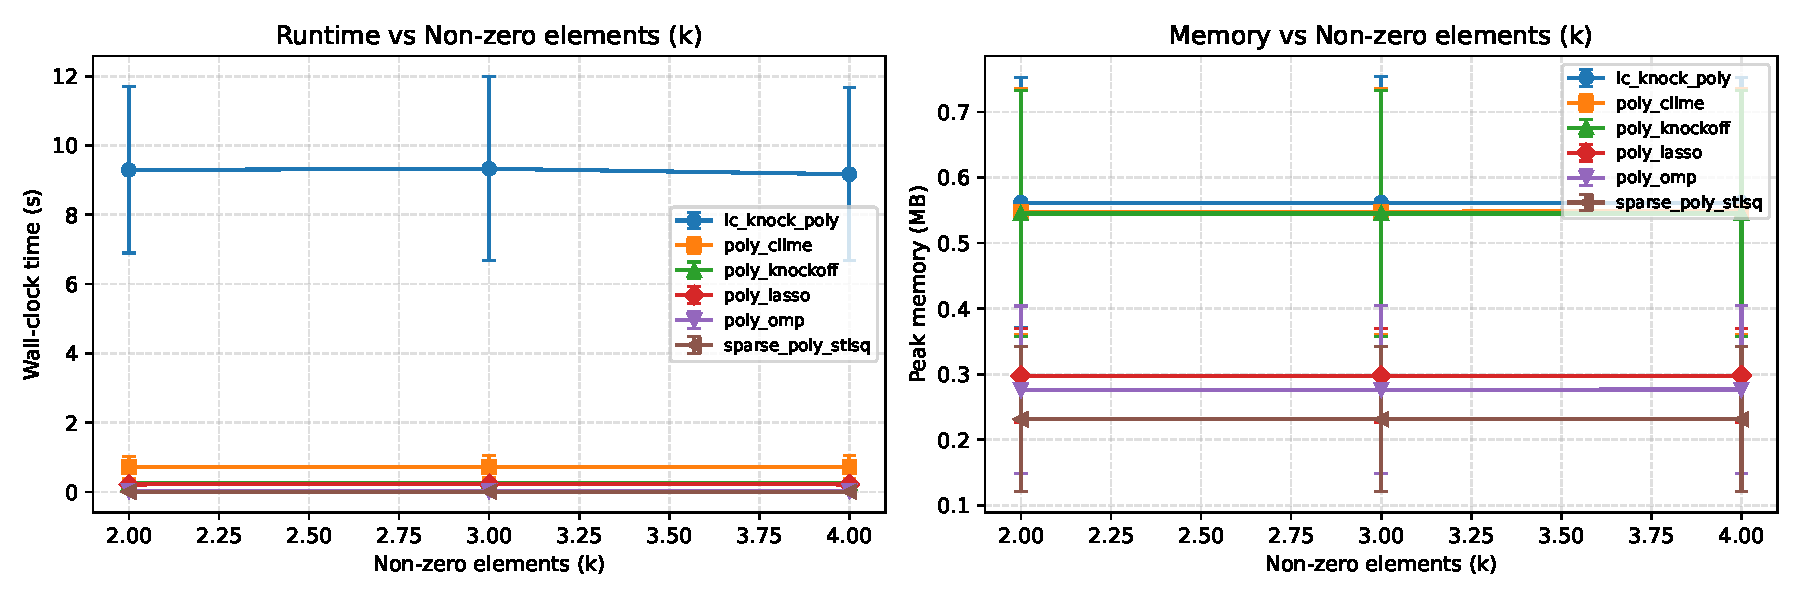
\includegraphics[width=0.9\textwidth]{figures/degree_nonzero_scalability_vs_k.pdf}
\caption{Scalability vs.\ k (degree nonzero sweep)}
\label{fig:degree_nonzero_scalability_vs_k}
\end{figure}


\begin{figure}[htbp]
\centering
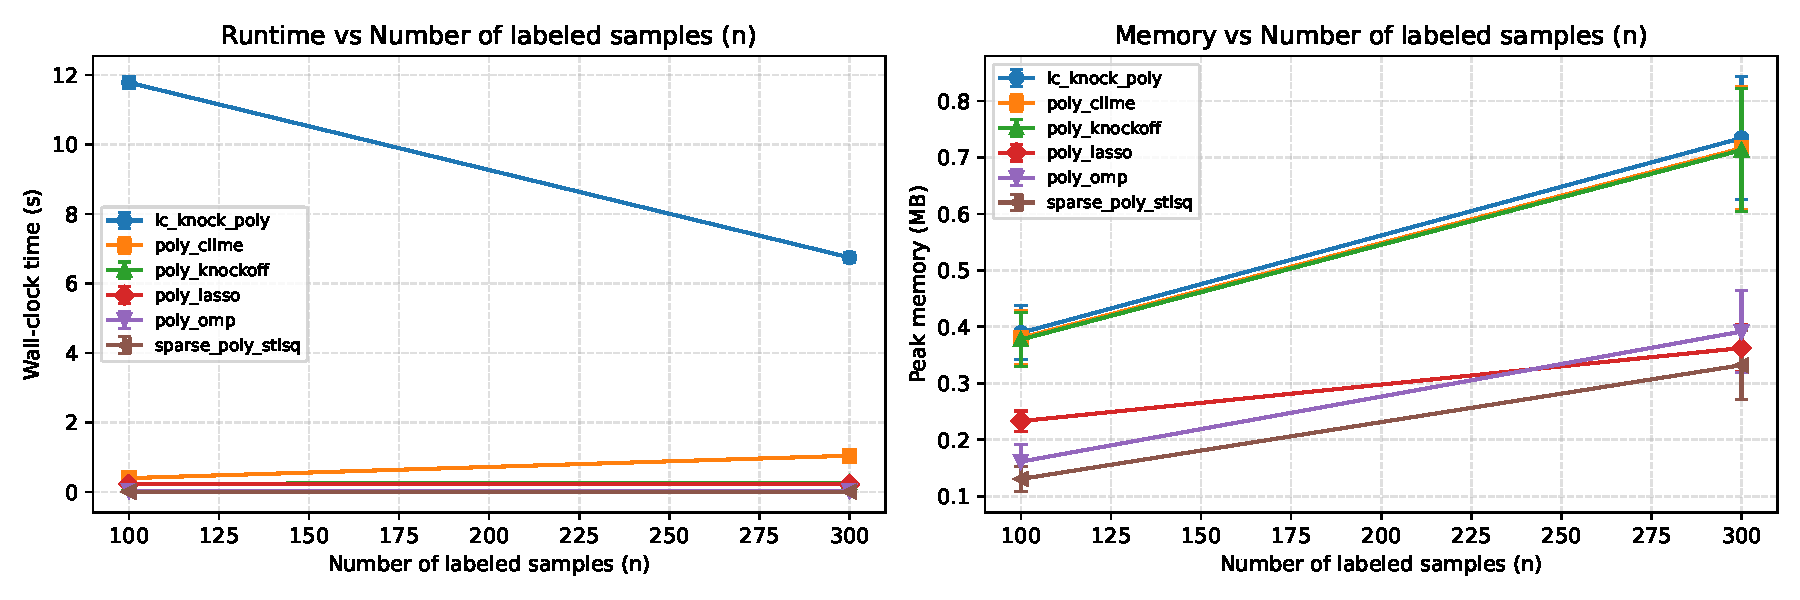
\includegraphics[width=0.9\textwidth]{figures/degree_nonzero_scalability_vs_n_labeled.pdf}
\caption{Scalability vs.\ n labeled (degree nonzero sweep)}
\label{fig:degree_nonzero_scalability_vs_n_labeled}
\end{figure}


\begin{figure}[htbp]
\centering
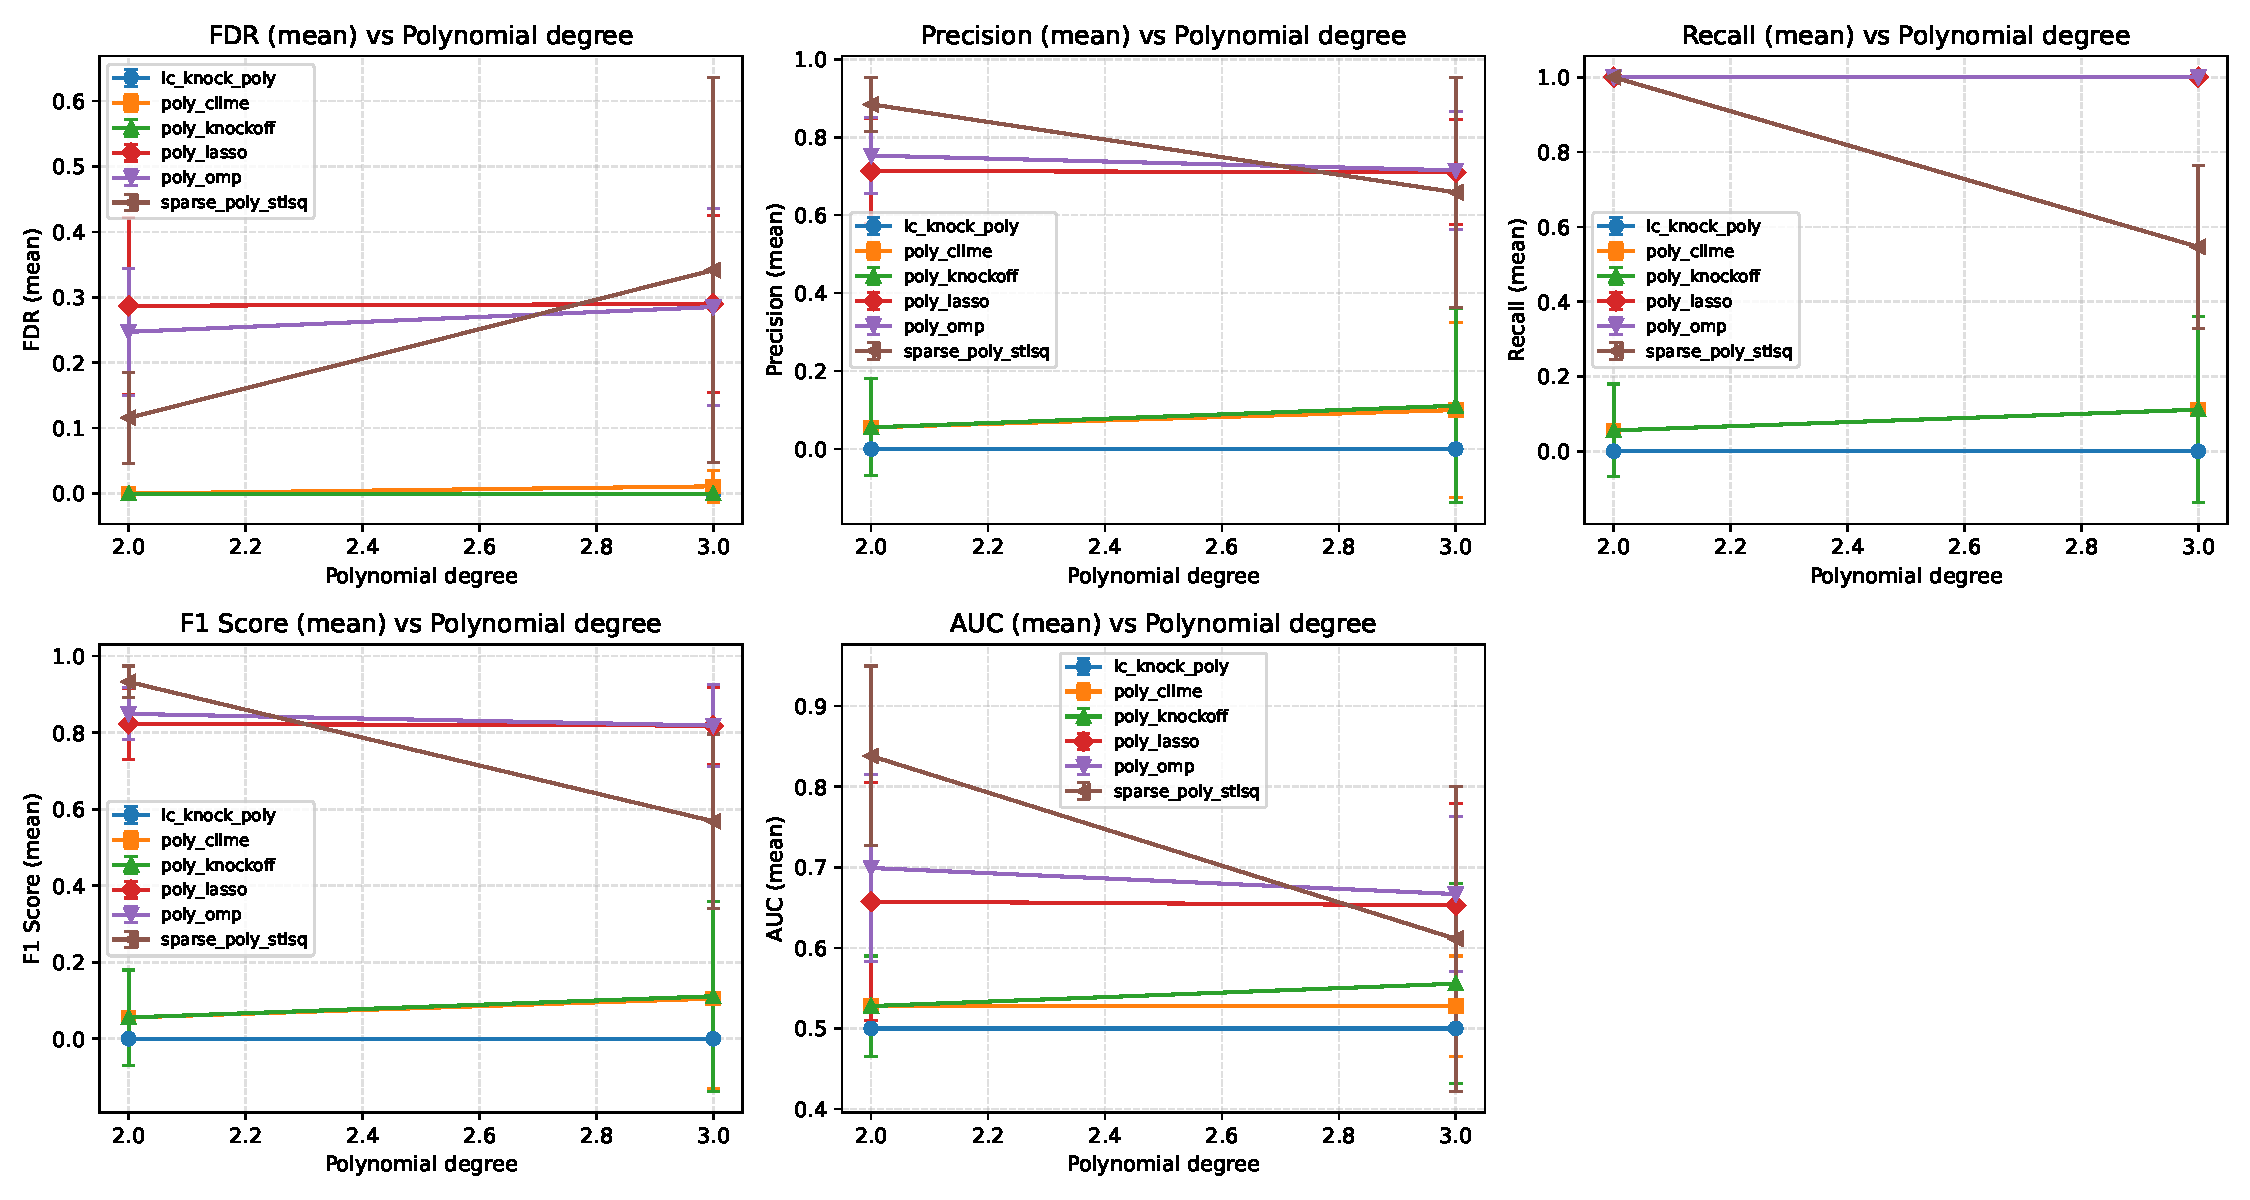
\includegraphics[width=0.9\textwidth]{figures/degree_nonzero_selection_metrics_vs_degree.pdf}
\caption{Selection Metrics vs.\ degree (degree nonzero sweep)}
\label{fig:degree_nonzero_selection_metrics_vs_degree}
\end{figure}


\begin{figure}[htbp]
\centering
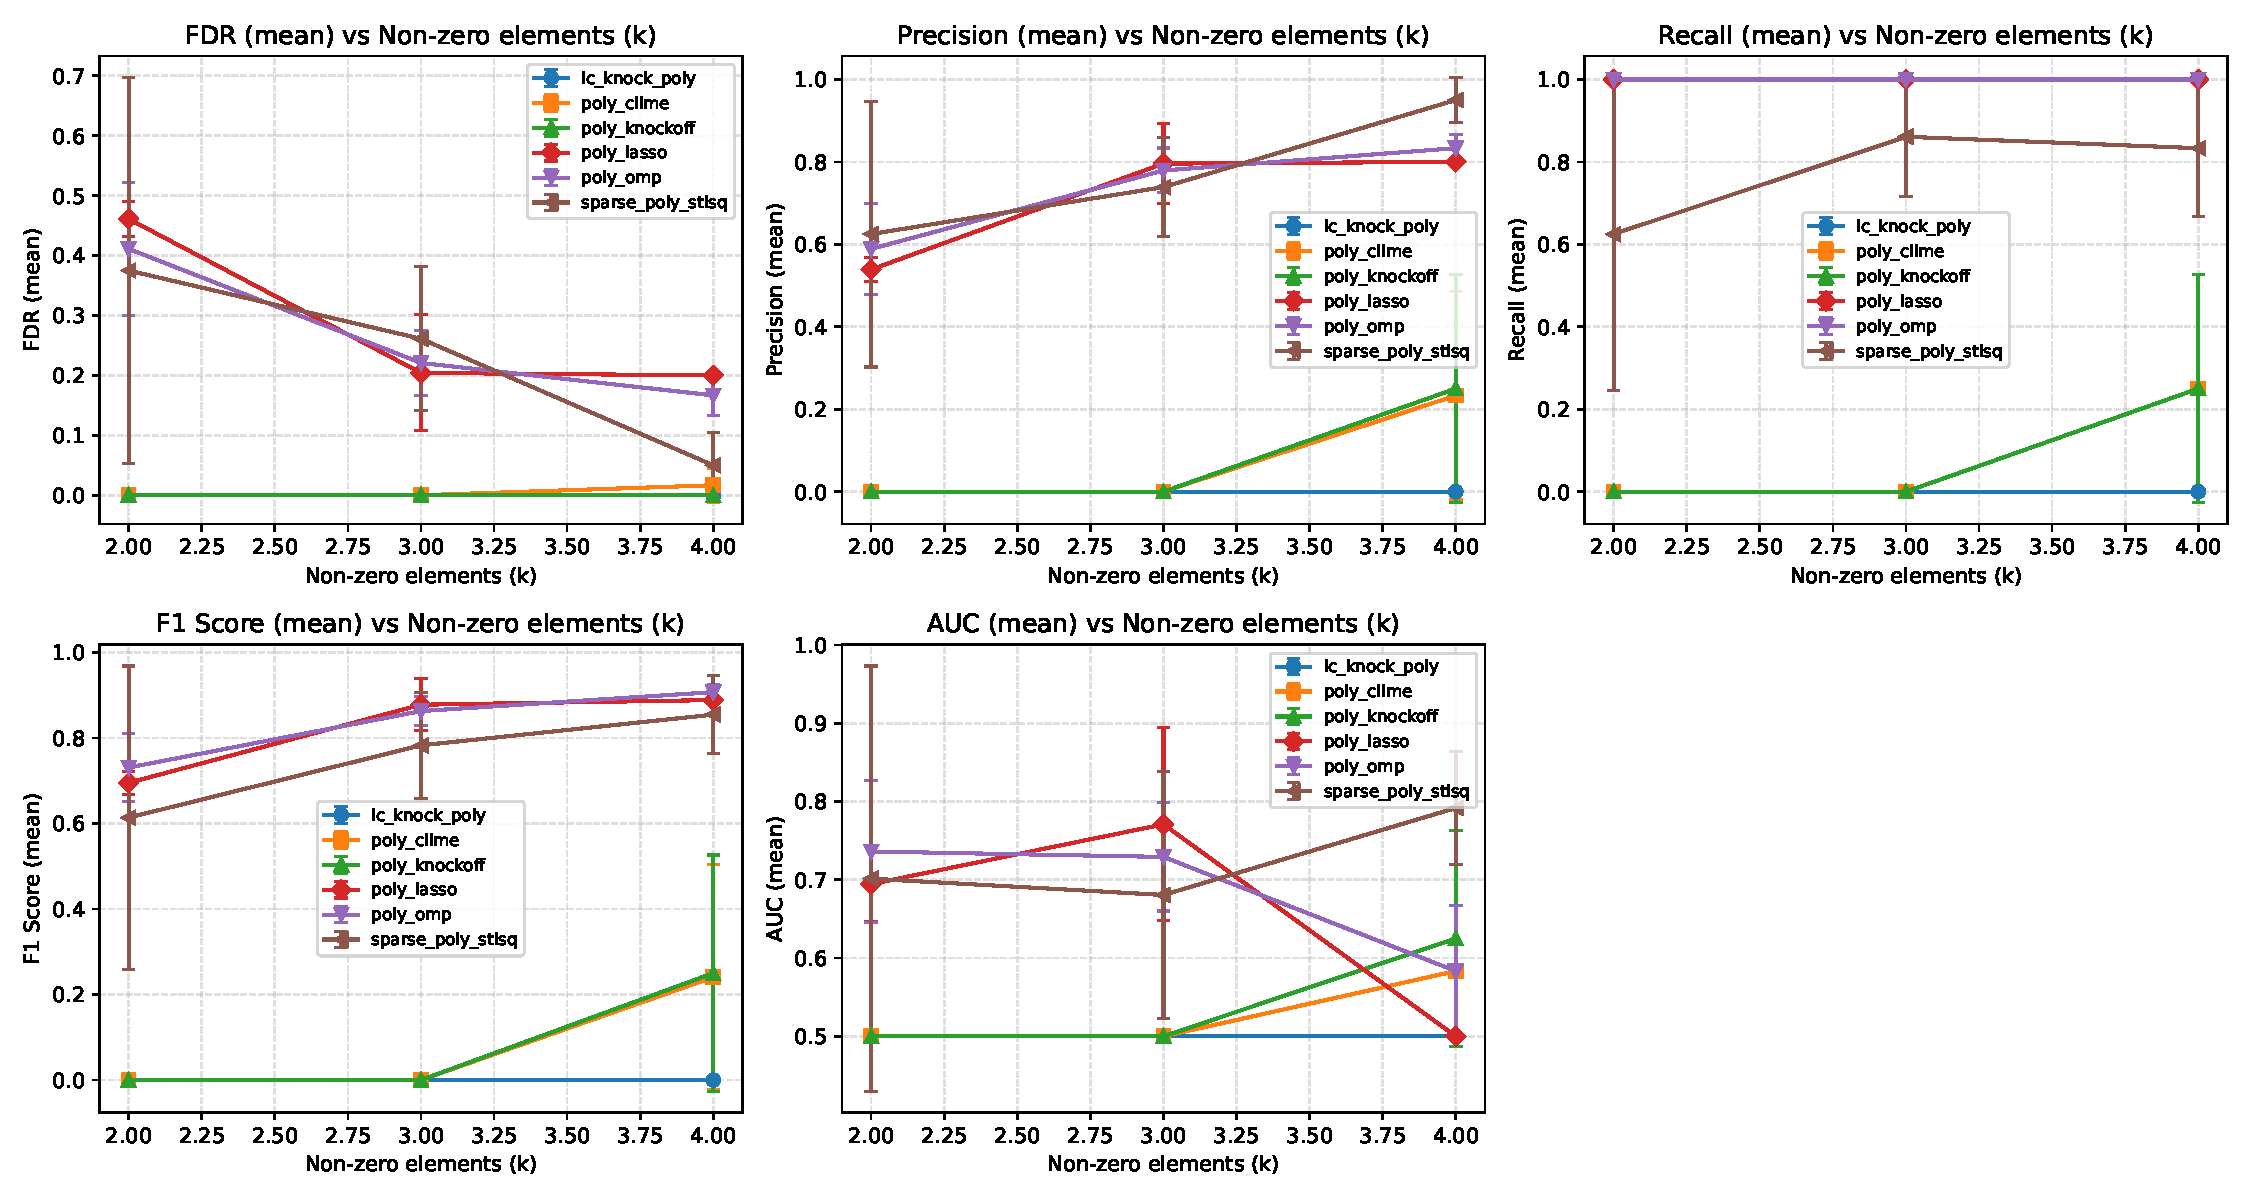
\includegraphics[width=0.9\textwidth]{figures/degree_nonzero_selection_metrics_vs_k.pdf}
\caption{Selection Metrics vs.\ k (degree nonzero sweep)}
\label{fig:degree_nonzero_selection_metrics_vs_k}
\end{figure}


\begin{figure}[htbp]
\centering
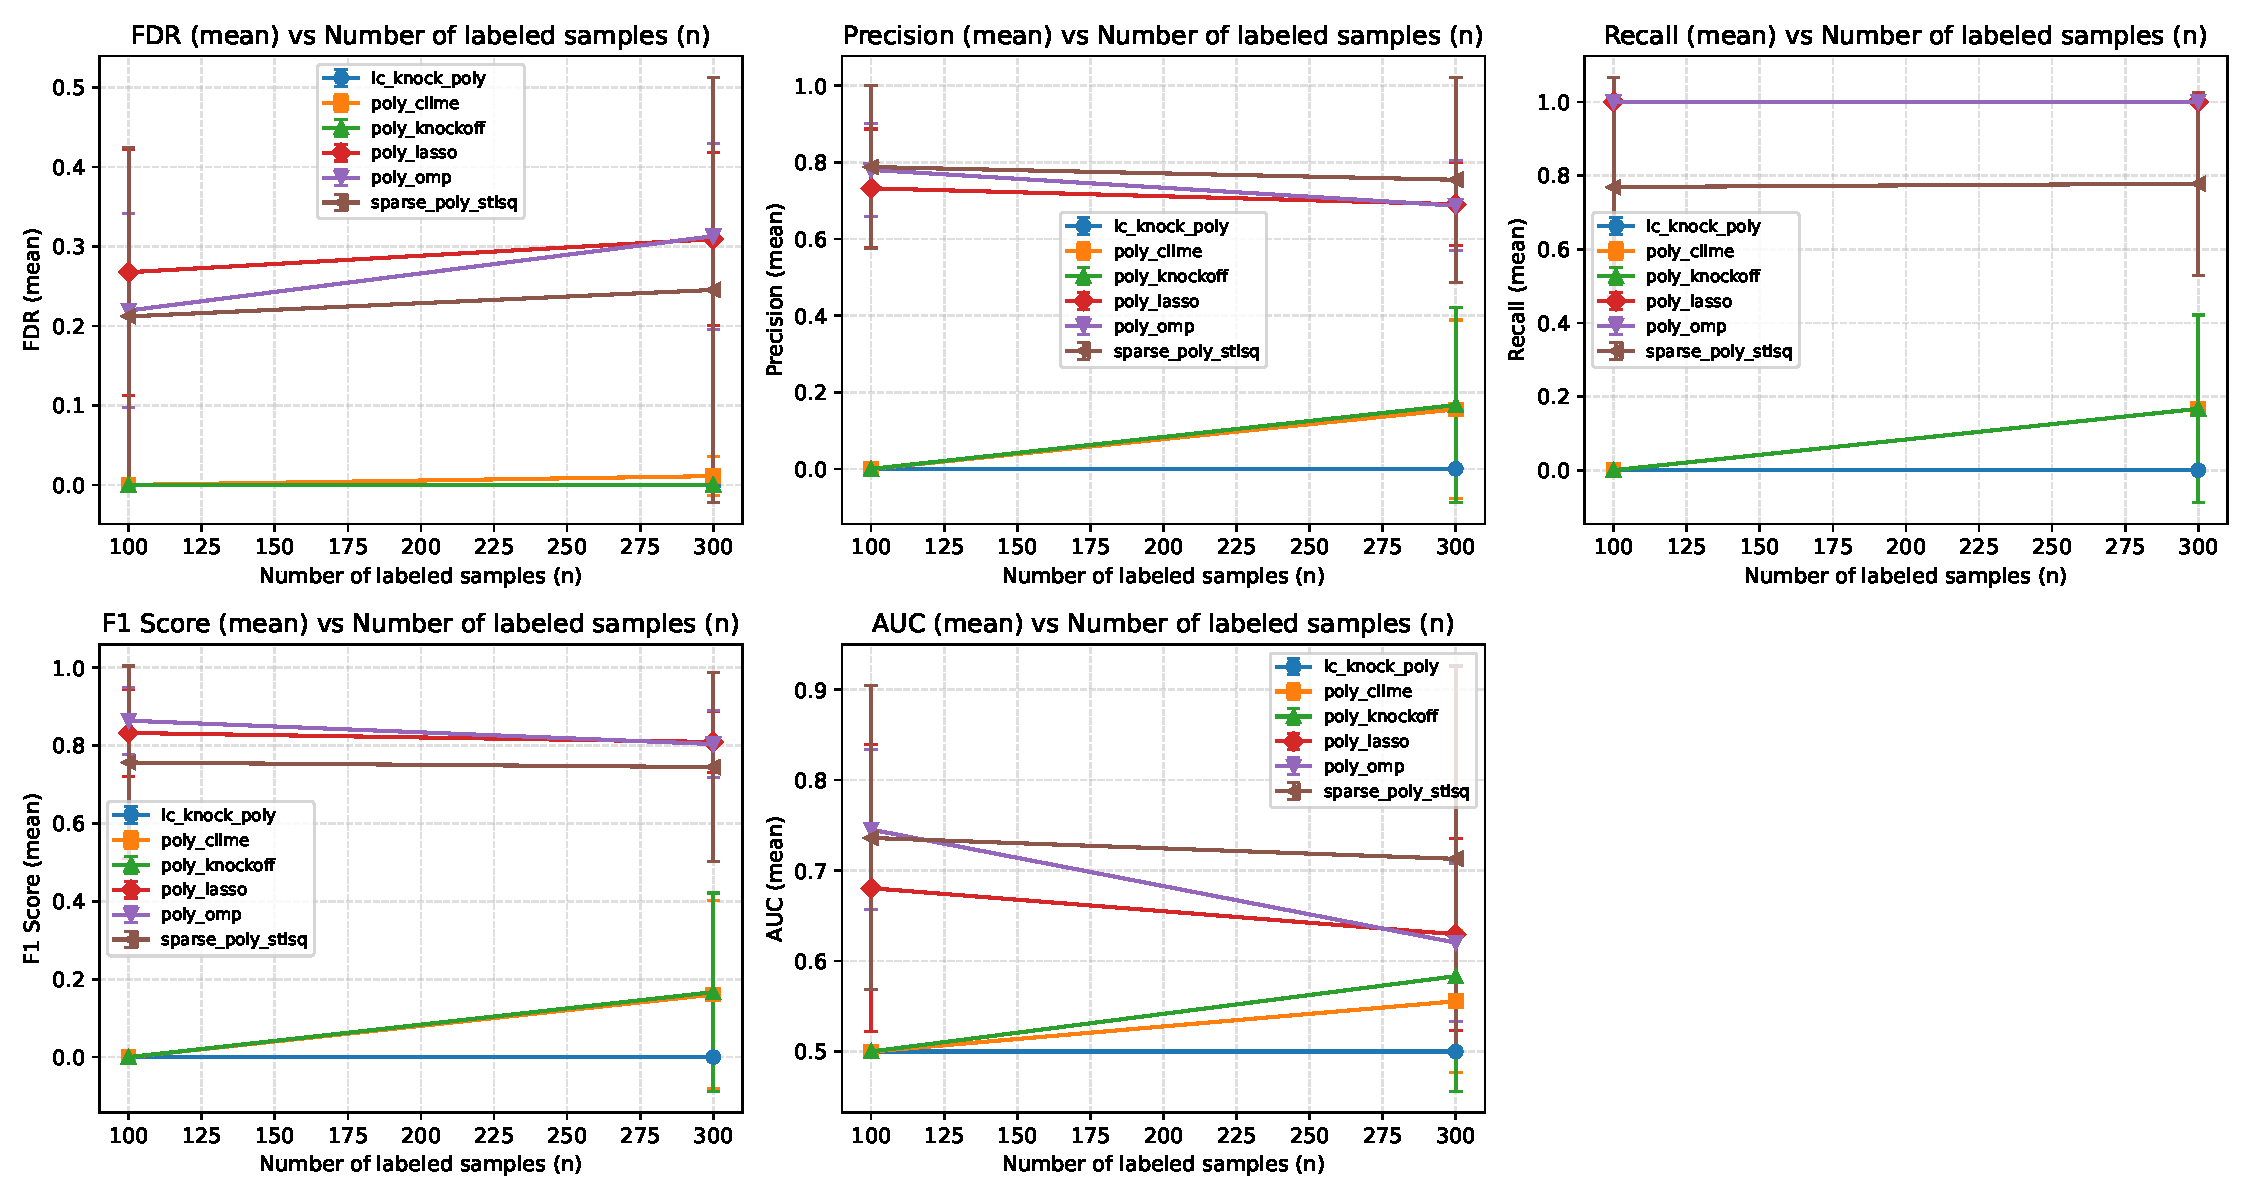
\includegraphics[width=0.9\textwidth]{figures/degree_nonzero_selection_metrics_vs_n_labeled.pdf}
\caption{Selection Metrics vs.\ n labeled (degree nonzero sweep)}
\label{fig:degree_nonzero_selection_metrics_vs_n_labeled}
\end{figure}


% ===================================================================
\section{Discussion}
\label{sec:discussion}

\begin{itemize}
  \item \textbf{FDR control}: IC-Knock-Poly targets \(Q = 0.10\).
        The empirical FDR is expected to remain at or below this threshold
        across all configurations when the model is well-specified.
  \item \textbf{TPR / Recall}: power typically increases with larger
        sample size \(n\) and decreases with higher sparsity \(k\) or
        polynomial degree \(d\).
  \item \textbf{Scalability}: wall-clock time and memory usage are shown
        in the scalability figures; note that IC-Knock-Poly's SDP
        construction is the dominant cost.
  \item \textbf{Baselines}: methods without formal FDR guarantees (e.g.\
        Poly-Lasso, Poly-OMP) often achieve higher TPR at the cost of
        inflated FDR.
  \item \textbf{Semi-supervised}: providing unlabeled data to
        IC-Knock-Poly can improve knockoff covariance estimation and
        thereby increase power (TPR) without inflating FDR.
\end{itemize}

% ===================================================================
\section{Conclusion}
\label{sec:conclusion}

This simulation study demonstrates that IC-Knockoff-PolyReg consistently
controls FDR at the specified level \(Q = 0.10\) across a range of
sample sizes, sparsity levels, and polynomial degrees, while maintaining
competitive predictive accuracy (R\textsuperscript{2}) compared with
standard baselines.

% ===================================================================
\end{document}
